\section{Presentation Markup}\label{PresentationMarkup}

\subsection{Introduction}

\subsubsection{Box Model}\label{BoxModel}

User agents must also follow the rules described in section 4.7.14
Embedded content, MathML of \cite{HTML5}, in particular the equivalence with
implicit {\tt mtext} and {\tt merror} to handle non-conforming MathML markup.

MathML elements have the following box model. The {\tt <math>} root may have
inline or block display, as suggested in section \ref{UAStylesheet}.
Tabular MathML elements have table, table-row and
table-cell display as discussed in section \ref{TabularMath}.
The {\tt <math>} and {\tt <mtd>} elements
generate an anonymous {\tt <mrow>} MathML box child that contains the boxes of
their children and use the box parameters below to layout this anonymous
{\tt <mrow>} box.
No line breaking can happen within MathML boxes and the min-content width is
equal to the max-content width, these are simply called the intrinsic width.
Each MathML box has the following parameters:

\begin{enumerate}
\item intrinsic width $W$.
\item logical width $w$, ascent above the origin $a$ and descent below the
  origin $b$. The height is then $a+b$.
\item ink ascent $A$ and descent $B$, corresponding to the exact box enclosing
  ink of text and bars within the MathML box.
\end{enumerate}

\begin{figure}
\centering
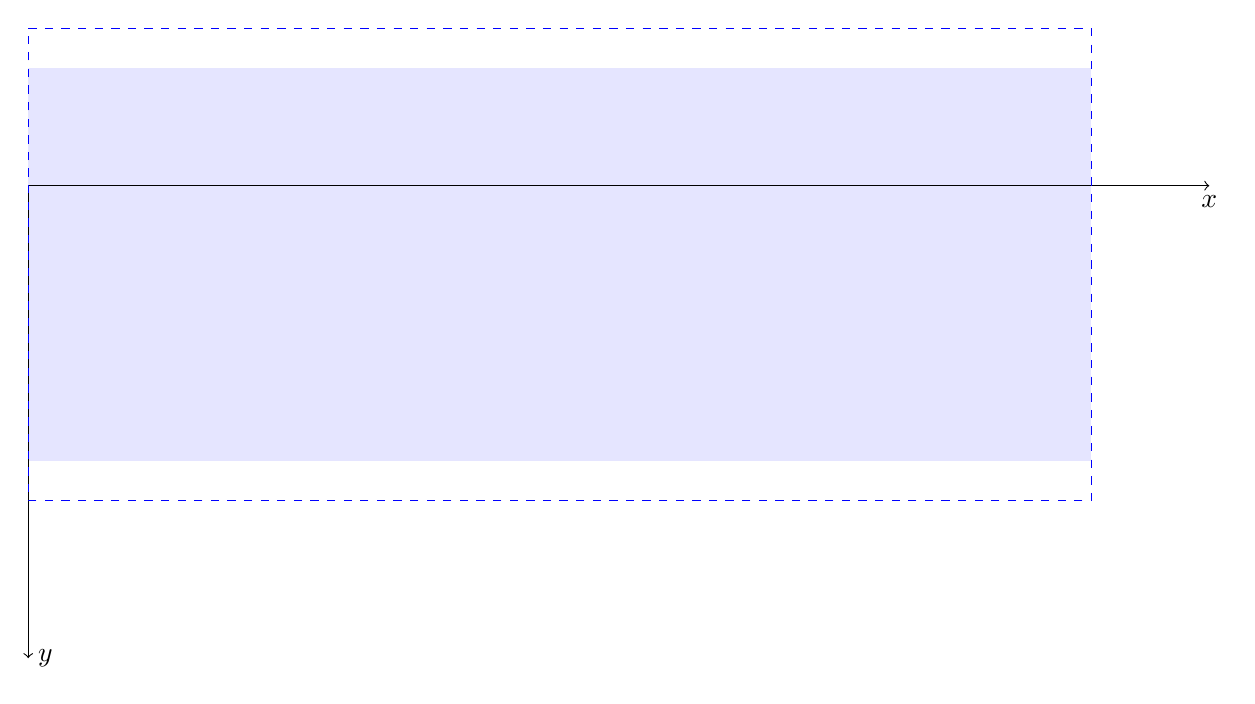
\begin{tikzpicture}[yscale=-1]
  \fill[blue!10] (0,-1.5) -- (13.5,-1.5) -- (13.5,3.5) -- (0,3.5) -- cycle;
  \draw[->] (0,0) -- (15,0) node[below] {$x$};
  \draw[->] (0,0) -- (0,6) node[right] {$y$};
  \draw[dashed,blue] (0,-2) -- (13.5,-2) -- (13.5,4) -- (0,4) -- cycle;
  \MathMLBox{0}{0}{1}{1}{red}
  \MathMLBoxMetrics{0}{0}{1}{1}{red}{1}
  \MathMLBox{6}{2}{1.5}{1}{green}
  \MathMLBoxMetrics{6}{2}{1.5}{1}{green}{2}
\end{tikzpicture}
\caption{Generic Box Model for MathML elements}
\label{fig:MathMLBoxModel}
\end{figure}

For MathML element containing only text nodes or foreign elements, we assume
that the content is simple enough to determine these values. For example,
in most case, this is just a single text node and $w = W$.
A MathML element containing only other MathML elements follow special rules to
layout their children at position $(x_i,y_i)$ with parameters
$W_i,w_i,a_i,b_i,A_i,B_i$. Then as a general rule, its box parameters are given
by taking the union of child boxes, that is:
%
$$w = \left(\max_{1 \leq i \leq n } {x_i + w_i}\right) -
      \left(\min_{1 \leq i \leq n} x_i\right)$$
$$W = \left(\max_{1 \leq i \leq n } {x_i + W_i}\right) -
      \left(\min_{1 \leq i \leq n} x_i\right)$$
$$a = \max_{1 \leq i \leq n } {a_i - y_i}$$
$$b = \max_{1 \leq i \leq n } {b_i + y_i}$$
$$A = \max_{1 \leq i \leq n } {A_i - y_i}$$
$$B = \max_{1 \leq i \leq n } {B_i + y_i}$$
%

Note that the schemas in this document are drawn assuming left-to-right
directionality. If the CSS {\tt direction} is set to right-to-left, then the
elements should be layout by making the $x$-axis pointing from right-to-left.
In this document, we use the terminology of \cite{MathML3}: ``leading''
means ``left'' in right-to-left and ``right'' in right-to-left mode, while
``trailing'' means ``right'' in right-to-left and ``left'' in right-to-left
mode.

The {\tt MathItalicsCorrectionInfo\lxAddClass{MATH}} table contains the italic
correction of some glyphs, which provides a measure of how slanted the
glyphs are (see figure \ref{fig:ItalicCorrection}). The
{\tt MathTopAccentAttachment\lxAddClass{MATH}} table also contains a reference
points that is used for the horizontal positioning of glyphs as an accent
(see figure \ref{fig:TopAccentAttachment}). In later sections, we
generalize this by claiming that all MathML boxes have italic correction
and top accent attachment values. The values for glyphs are used to try and
extend to token elements or to special boxes that do not change child metrics.
Otherwise fallback values are used: 0 for italic correction and half
the width of the box for top accent attachment.

\begin{figure}
\centering
  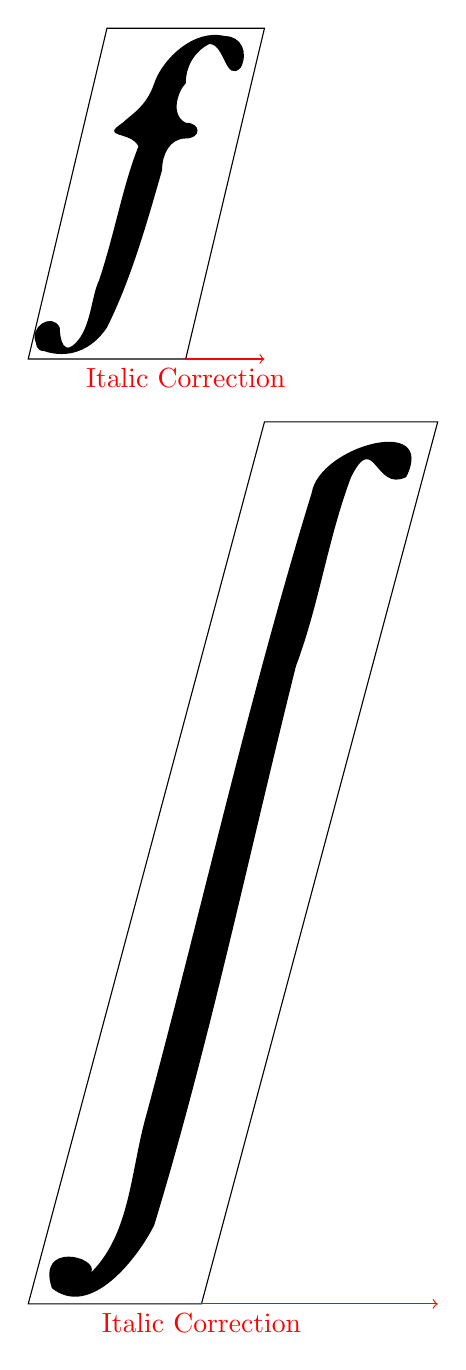
\begin{tikzpicture}[yscale=-1]

    \begin{scope}[xscale=.1,yscale=.1]
    \fill[black] (1,40) .. controls (0,38) and (3,36) .. (4,38) .. controls (4,38) and (4,42) .. (6,40) .. controls (8,38) and (8,34) .. (9,32) .. controls (11,26) and (12,20) .. (14,15) .. controls (13,13) and (9,14) .. (12,12) .. controls (13,11) and (15,10) .. (16,7) .. controls (17,4) and (21,0) .. (25,1) .. controls (27,1) and (28,3) .. (27,5) .. controls (25,7) and (25,2) .. (23,2) .. controls (21,3) and (20,5) .. (20,7) .. controls (19,8) and (18,11) .. (20,12) .. controls (22,12) and (22,14) .. (20,14) .. controls (18,14) and (17,16) .. (17,18) .. controls (15,25) and (13,32) .. (10,38) .. controls (8,41) and (5,42) .. (2,41) .. controls (1,41) and (1,40) .. (1,40) -- cycle;
    \draw[black] (10,0) -- (30,0) -- (20,42) -- (0,42) -- cycle;
    \draw[red,->] (20,42) node[below]{Italic Correction} -- (30,42);
    \end{scope}

    \begin{scope}[shift={(0,5)},xscale=.1,yscale=.1]
    \fill[black] (3,110) .. controls (1,104) and (9,106) .. (8,108) .. controls (13,103) and (13,95) .. (15,88) .. controls (22,62) and (28,35) .. (36,9) .. controls (37,3) and (52,-1) .. (48,7) .. controls (44,9) and (44,1) .. (41,7) .. controls (38,15) and (37,23) .. (34,31) .. controls (28,55) and (23,79) .. (16,102) .. controls (14,106) and (8,114) .. (3,110) -- cycle;
    \draw[black] (30,0) -- (52,0) -- (22,112) -- (0,112) -- cycle;
    \draw[red,->] (22,112) node[below]{Italic Correction} -- (52,112);
    \end{scope}
\end{tikzpicture}
\caption{Examples of italic correction for italic f and large integral}
\label{fig:ItalicCorrection}
\end{figure}

\begin{figure}
\centering
  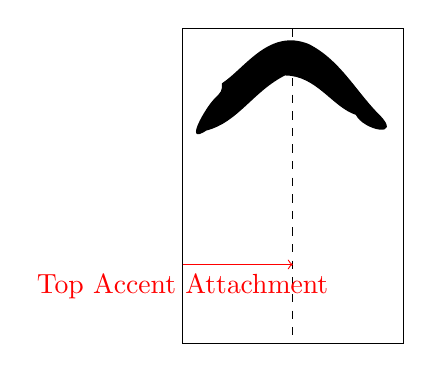
\begin{tikzpicture}[yscale=-1]
    \begin{scope}[xscale=.1,yscale=.1]
    \fill[black]
    (5,7) .. controls (8,5) and (11,0) .. (16,2) .. controls (20,4) and (22,8) .. (25,11) .. controls (28,14) and (23,13) .. (22,11) .. controls (19,10) and (17,6) .. (13,6) .. controls (9,8) and (7,12) .. (3,13) .. controls (0,15) and (3,10) .. (4,9) .. controls (5,8) and (5,8) .. (5,7) -- cycle;
    \draw[black] (0,0) rectangle (28,40);
    \draw[black,dashed](14,0) -- (14,40);
    \draw[red,->] (0,30) node[below]{Top Accent Attachment} -- (14,30);
    \end{scope}
  \end{tikzpicture}
\caption{Example of top accent attachment for a circumflex accent}
\label{fig:TopAccentAttachment}
\end{figure}

The present document assumes that $W,w,a,b,A,B$, italic correction
and top accent attachment are nonnegative values. If computations result
in negative values, then they must be interpreted as being zero.
Note that some MathML elements such as {\tt mspace} or {\tt mpadded} may set box
dimensions to negative values.

\subsubsection{Layout Steps}\label{LayoutSteps}

For compatibility with HTML5 rendering, the MathML layout is performed in two
independent steps:

\begin{enumerate}
\item In the first step, we determine the intrinsic width $W$ of MathML boxes.
  To do so we just follow the description given in this document for each
  MathML box. We rely on vertical positions $x$ as well as values for
  italic correction and top accent attachment. However, we ignore any vertical
  positioning or metrics.
\item In the second step, we do the final layout of MathML boxes following
  the description given in this document. We obtain all the box metrics,
  including the actual width $w$, vertical metrics $a,b,A,B$ and
  vertical positions $y$.
\end{enumerate}

In order to perform the first step independently of the second one, the
horizontal metrics must not depend on the vertical metrics. As described in
section \ref{mpadded}, this adds some restrictions on the possible pseudo-units
of the {\tt mpadded} element. As indicated in section \ref{Operators},
the width of size variants or of the glyph assembly used for vertical stretchy
operators may depend on the target size to cover. Taking the maximum widths
for all these size variants or for the glyph assembly during the first step
makes the intrinsic width independent of the target size but may lead to a
small over-estimation.

Each of this step is done recursively: the metrics of a given MathML box
are determined from those of the child boxes. User agents must implement
the ``Exception for embellished operators'' described in \cite{MathML3}.
This means that the actual stretching of operators described in section
\ref{Operators} may be ``delayed'' until we reach the top of its embellished
operator subtree. We then have to apply the current operation again
to this embellished operator (intrinsic width determination or layout).
Fortunately, such embellished operator subtrees are not deep in practice.

This document does not require support for operator stretching in table cells.
The ``delayed'' stretching of all operators must then be performed when we
arrive at the anonymous {\tt <mrow>} child of {\tt <math>} and {\tt <mtd>}
elements.
That way, the intrinsic width of this anonymous {\tt <mrow>} is well-defined
for the layout of {\tt mtable} elements and of the containers of the
{\tt <math>} element. Similarly, the final layout of this anonymous
{\tt <mrow>} is already done when we want to perform the one of its ancestors.

\subsection{Token Elements}

\subsubsection{Using images to represent symbols {\tt <mglyph/>}}

The MathML specification describes {\tt mglyph} as follows \cite{MathML3}:
%
\begin{quote}
The mglyph element provides a mechanism for displaying images to represent
non-standard symbols.
\end{quote}

This document does define any layout algorithm for the {\tt mglyph}
element. User agents may just ignore it.

\subsubsection{Identifier {\tt <mi>}}\label{Identifier}

The MathML specification describes {\tt mi} as follows \cite{MathML3}:
%
\begin{quote}
  An {\tt mi} element represents a symbolic name or arbitrary text that should
  be rendered as an identifier.
\end{quote}

In general, the {\tt mi} element must be treated the same as the {\tt mtext}
element. However, when the {\tt mathvariant} on an {\tt mi} element is
{\tt none} and the {\tt mi} content is made of a single character then the
element must behave as if {\tt mathvariant} was actually set to {\tt italic}.

\subsubsection{Number {\tt <mn>}}

The MathML specification describes {\tt mn} as follows \cite{MathML3}:
%
\begin{quote}
  An {\tt mn} element represents a "numeric literal" or other data that should
  be rendered as a numeric literal.
\end{quote}

For the layout algorithm described in this document, the
{\tt mn} element must be treated the same as the {\tt mtext} element.

\subsubsection{Operator, Fence, Separator or Accent {\tt <mo>}}\label{Operators}

The MathML specification describes {\tt mo} as follows \cite{MathML3}:
%
\begin{quote}
  An {\tt mo} element represents an operator or anything that should be
  rendered as an operator.
\end{quote}

Many properties of an {\tt mo} element can be specified via attribute on
that element. The default value of the {\tt form} of an {\tt mo} element is
obtained as described in section ``Default value of the form attribute'' of
\cite{MathML3}. From the {\tt form} and the text content, we can deduce other
default values from the operator dictionary or use the fallback values given
in ``Dictionary-based attributes'' of \cite{MathML3}.

The leading space {\tt lspace} and trailing space {\tt rspace} must be added on
each side of the {\tt mo} element (or its outermost embellished ancestor).

In most cases, the {\tt mo} element is treated as an {\tt mtext} element.
However, when an {\tt mo} element with a single character must be displayed as
a large operator then instead we use the {\tt MathVariants\lxAddClass{MATH}}
table to try and find a glyph of height at least
{\tt DisplayOperatorMinHeight\lxAddClass{MATH}}
(figure \ref{fig:LargeOpVariant}). If none is found, we fallback to the
largest one. Because this parameter does not always give
the best size, user agents may also use the following heuristic: ensure
that the large variant height is at least $2$ times as large as the base height
for integrals and $\sqrt{2}$ times as large as the base height for other
operators.

\begin{figure}
\centering
  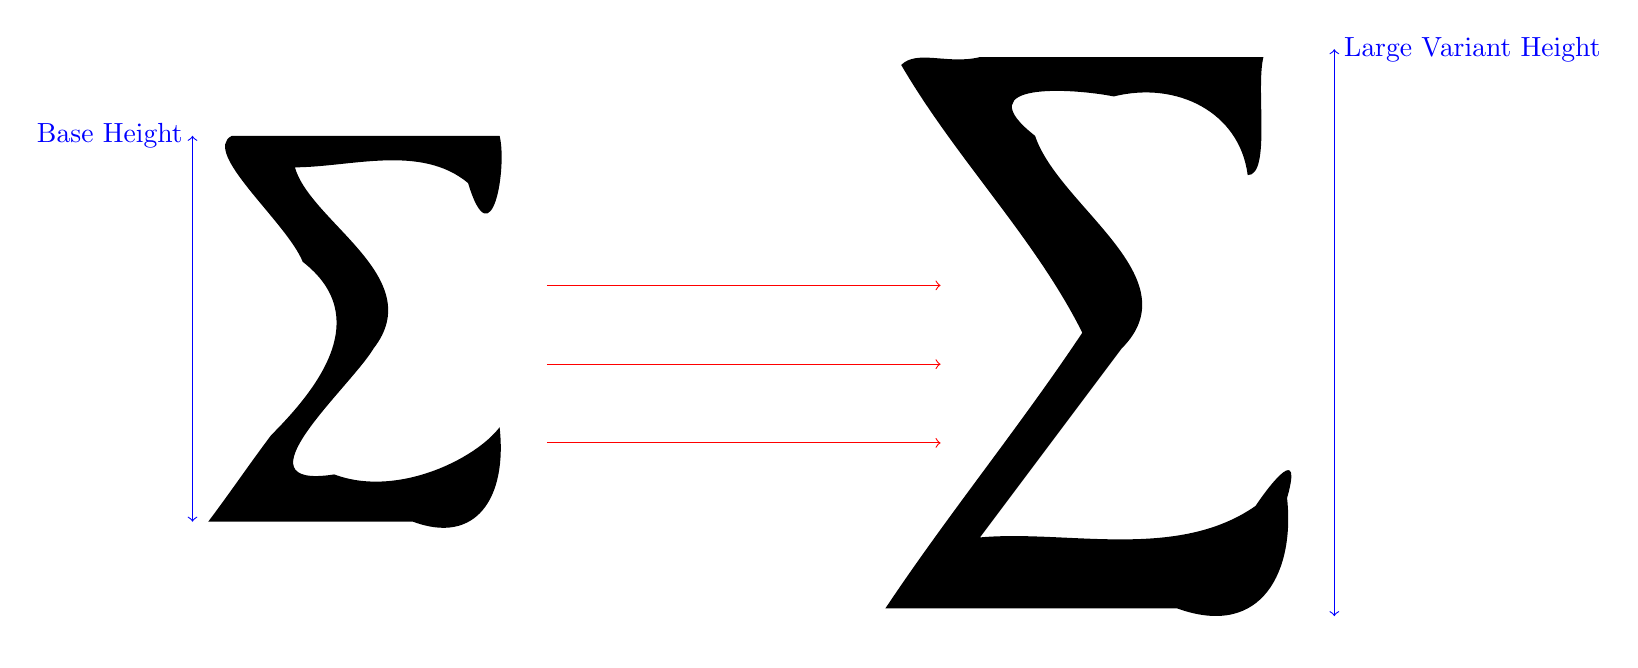
\begin{tikzpicture}[yscale=-1]

    \begin{scope}[xscale=.1,yscale=.1]
    \fill[black](63,71) .. controls (71,59) and (80,48) .. (88,36) .. controls (82,24) and (72,14) .. (65,2) .. controls (67,0) and (71,2) .. (75,1) .. controls (87,1) and (99,1) .. (111,1) .. controls (110,5) and (112,16) .. (109,16) .. controls (108,8) and (100,4) .. (92,6) .. controls (87,5) and (73,4) .. (82,11) .. controls (85,20) and (102,29) .. (93,38) .. controls (87,46) and (81,54) .. (75,62) .. controls (86,61) and (100,65) .. (110,58) .. controls (112,55) and (116,50) .. (114,57) .. controls (115,66) and (111,75) .. (100,71) .. controls (88,71) and (75,71) .. (63,71);
    \draw[blue,<->] (-25,11)node[left]{Base Height} -- (-25, 60);

    \draw[red,->] (20,30) -- (70,30);
    \draw[red,->] (20,40) -- (70,40);
    \draw[red,->] (20,50) -- (70,50);

    \begin{scope}[shift={(-25,0)}]
    \fill[black](10,49) .. controls (16,43) and (23,34) .. (14,27) .. controls (12,22) and (1,13) .. (5,11) .. controls (16,11) and (27,11) .. (39,11) .. controls (40,15) and (38,27) .. (35,17) .. controls (29,12) and (20,15) .. (13,15) .. controls (15,22) and (30,29) .. (23,38) .. controls (20,43) and (5,56) .. (18,54) .. controls (26,57) and (36,52) .. (39,48) .. controls (40,57) and (36,63) .. (28,60) .. controls (19,60) and (10,60) .. (2,60) .. controls (5,56) and (7,53) .. (10,49);
    \draw[blue,<->] (145,0)node[right]{Large Variant Height} -- (145, 72);
    \end{scope}
    \end{scope}
\end{tikzpicture}
\caption{Base and displaystyle sizes of the summation symbol}
\label{fig:LargeOpVariant}
\end{figure}

When an {\tt mo} element with a single character must be displayed as a
horizontal or vertical
operator then instead of displaying the normal character we use
the {\tt MathVariants\lxAddClass{MATH}} table to try and find a glyph
that has at least the desired size or an assembly from several glyphs
to cover at least the desired size
(figure \ref{fig:StretchyOperators}). The rules for vertical stretching
are a bit more complicated and are described in section
``Vertical Stretching Rules'' of \cite{MathML3}. If the operator has property
{\tt symmetric="true"}, it must be stretched symmetrically with respect to
the axis height, using the {\tt AxisHeight\lxAddClass{MATH}} value as the math
axis. Figure \ref{fig:SymmetricNonSymmetricOperators} compares the symmetric
and non-symmetric stretching.

The size variant or construction used for vertical stretchy operators will
depend on the target size to cover. To determine the intrinsic
width $W$ of the operator, we consider the maximum of all possible widths
for the base size, size variants and construction available for the given
operator. It is assumed that the width of the
operator is almost independent of the stretch size, which is the case in
practice for most math fonts and operators.

\begin{figure}
\centering
  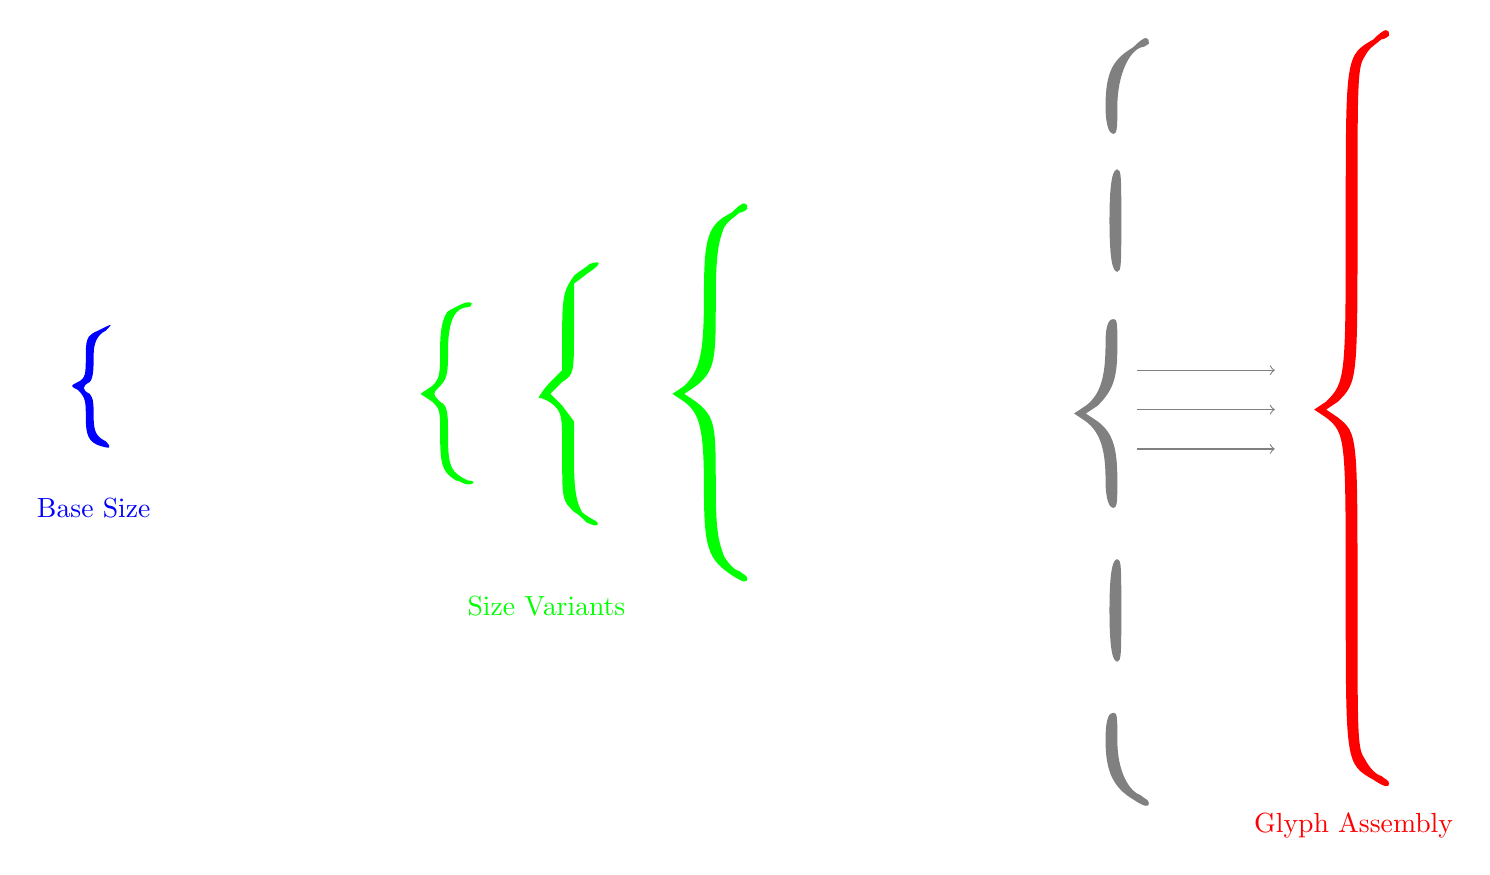
\begin{tikzpicture}[yscale=-1]

    \begin{scope}[xscale=.05,yscale=.05]

      \fill[blue] (11,109) .. controls (9,108) and (8,107) .. (8,102) .. controls (8,98) and (8,97) .. (6,95) .. controls (4,94) and (4,94) .. (6,93) .. controls (8,92) and (8,91) .. (8,86) .. controls (8,81) and (9,81) .. (11,80) .. controls (15,78) and (15,78) .. (13,80) .. controls (11,81) and (10,83) .. (10,86) .. controls (10,89) and (10,92) .. (9,93) .. controls (7,94) and (7,95) .. (9,96) .. controls (10,97) and (10,99) .. (10,102) .. controls (10,106) and (11,107) .. (13,108) .. controls (15,110) and (14,110) .. (11,109);
      \draw[blue] (10,120) node[below]{Base Size};

      \fill[green] (172,142) .. controls (166,138) and (165,135) .. (165,120) .. controls (165,105) and (164,101) .. (160,98) -- (157,96) -- (160,94) .. controls (164,90) and (165,86) .. (165,71) .. controls (165,56) and (166,53) .. (172,50) .. controls (175,47) and (176,47) .. (176,49) .. controls (176,49) and (175,50) .. (174,50) .. controls (173,51) and (171,52) .. (170,54) .. controls (169,57) and (168,59) .. (168,72) .. controls (168,87) and (168,90) .. (163,94) -- (160,96) -- (163,98) .. controls (168,102) and (168,104) .. (168,120) .. controls (168,132) and (169,134) .. (170,137) .. controls (171,139) and (173,141) .. (174,141) .. controls (175,142) and (176,142) .. (176,143) .. controls (176,144) and (175,144) .. (172,142);
      \fill[green] (136,129) .. controls (135,129) and (134,127) .. (132,126) .. controls (129,123) and (129,123) .. (129,112) .. controls (129,102) and (129,101) .. (127,99) .. controls (126,98) and (124,97) .. (123,97) .. controls (123,97) and (124,95) .. (126,93) -- (129,90) -- (129,79) .. controls (129,70) and (130,69) .. (132,66) .. controls (133,65) and (135,64) .. (136,63) .. controls (139,62) and (139,63) .. (136,65) -- (132,68) -- (132,79) .. controls (132,91) and (132,91) .. (129,93) -- (126,96) -- (129,99) -- (132,103) -- (132,113) .. controls (132,122) and (133,124) .. (134,126) .. controls (135,127) and (137,128) .. (137,128) .. controls (139,129) and (138,130) .. (136,129);
      \fill[green] (102,118) .. controls (99,116) and (98,115) .. (98,107) .. controls (98,100) and (98,100) .. (96,98) -- (93,96) -- (96,94) .. controls (98,92) and (98,91) .. (98,84) .. controls (98,79) and (99,76) .. (100,75) .. controls (102,74) and (105,72) .. (106,73) .. controls (106,73) and (106,74) .. (105,74) .. controls (102,74) and (100,77) .. (100,85) .. controls (100,90) and (100,92) .. (98,94) .. controls (96,96) and (96,96) .. (98,98) .. controls (100,99) and (100,101) .. (100,107) .. controls (100,115) and (101,116) .. (105,118) .. controls (107,118) and (107,119) .. (105,119) .. controls (104,119) and (103,118) .. (102,118);
      \draw[green] (125,145) node[below]{Size Variants};

      \fill[gray] (274,199) .. controls (269,196) and (267,192) .. (267,184) .. controls (267,178) and (268,177) .. (269,177) .. controls (270,177) and (270,178) .. (270,184) .. controls (270,192) and (273,197) .. (276,198) .. controls (277,199) and (278,199) .. (278,200) .. controls (278,201) and (277,201) .. (274,199);
      \fill[gray] (268,151) .. controls (268,140) and (269,138) .. (270,138) .. controls (271,138) and (271,140) .. (271,151) .. controls (271,162) and (271,164) .. (270,164) .. controls (269,164) and (268,162) .. (268,151);
      \fill[gray] (267,118) .. controls (267,111) and (266,106) .. (262,103) -- (259,101) --  (262,99) .. controls (266,96) and (267,91) .. (267,83) .. controls (267,78) and (268,77) .. (269,77) .. controls (270,77) and (270,78) .. (270,84) .. controls (270,92) and (269,95) .. (265,99) -- (262,101) -- (265,103) .. controls (269,106) and (270,110) .. (270,118) .. controls (270,123) and (270,125) .. (269,125) .. controls (268,125) and (267,123) .. (267,118);
      \fill[gray](268,52) .. controls (268,41) and (269,39) .. (270,39) .. controls (271,39) and (271,41) .. (271,52) .. controls (271,63) and (271,65) .. (270,65) .. controls (269,65) and (268,63) .. (268,52);
      \fill[gray] (267,23) .. controls (267,14) and (269,11) .. (274,8) .. controls (277,5) and (278,5) .. (278,7) .. controls (278,7) and (277,8) .. (276,8) .. controls (273,9) and (270,15) .. (270,23) .. controls (270,28) and (270,30) .. (269,30) .. controls (268,30) and (267,28) .. (267,23);

      \draw[->,color=gray] (275,90) -- (310,90);
      \draw[->,color=gray] (275,100) -- (310,100);
      \draw[->,color=gray] (275,110) -- (310,110);

      \fill[red] (335,194) .. controls (328,190) and (328,190) .. (328,148) .. controls (328,107) and (328,106) .. (323,102) -- (320,100) -- (323,98) .. controls (328,93) and (328,92) .. (328,51) .. controls (328,10) and (328,10) .. (335,6) .. controls (338,3) and (339,3) .. (339,5) .. controls (339,5) and (338,6) .. (337,6) .. controls (336,7) and (334,8) .. (333,10) .. controls (331,13) and (331,15) .. (331,52) .. controls (331,93) and (331,93) .. (326,98) -- (323,100) -- (326,102) .. controls (331,106) and (331,106) .. (331,148) .. controls (331,185) and (331,186) .. (333,189) .. controls (334,191) and (336,193) .. (337,193) .. controls (338,194) and (339,194) .. (339,195) .. controls (339,196) and (338,196) .. (335,194) -- cycle;
      \draw[red] (330,200) node[below]{Glyph Assembly};
    \end{scope}
    \end{tikzpicture}
\caption{Base size, size variants and glyph assembly for the left brace}
\label{fig:StretchyOperators}
\end{figure}

\begin{figure}
\centering
  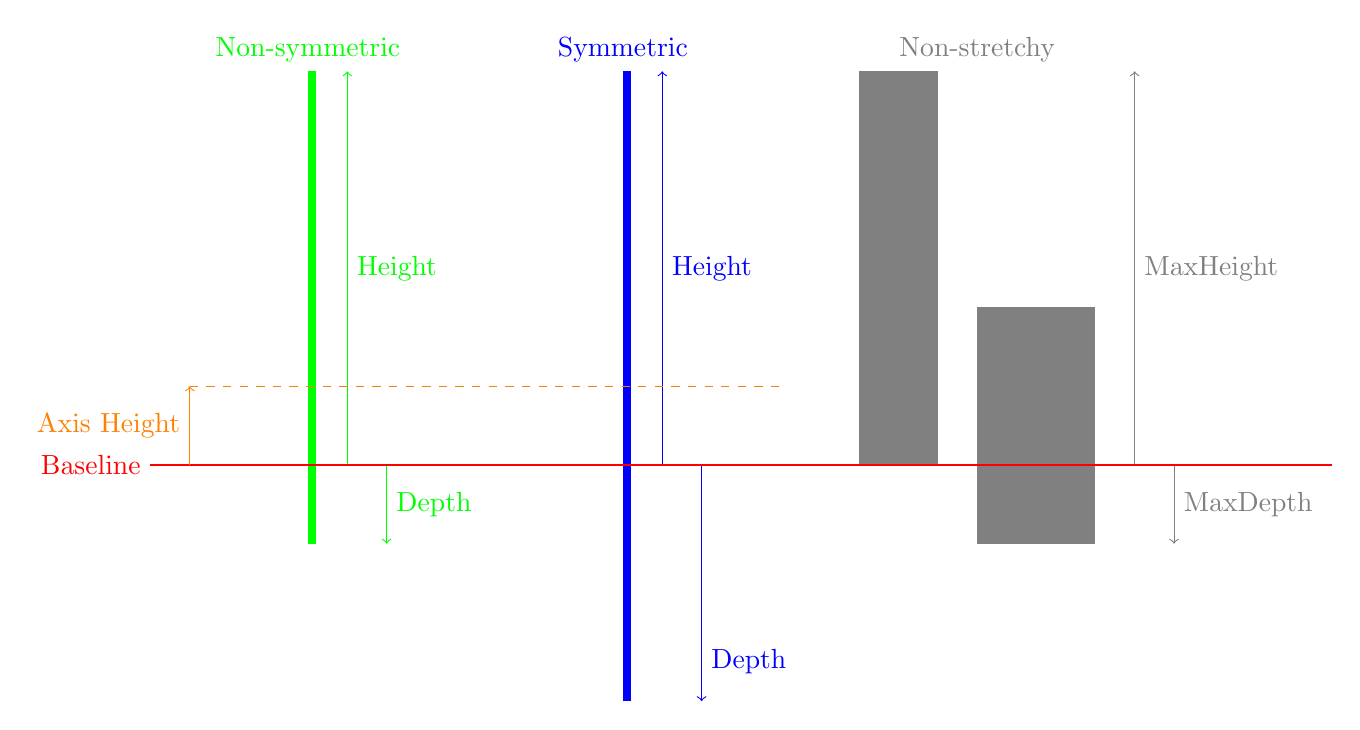
\begin{tikzpicture}[yscale=-1]
  \fill[green](2,-5) node[above]{Non-symmetric} rectangle (2.1,1);
  \draw[green,->](2.5,0) -- (2.5, -2.5) node[right]{Height} -- (2.5,-5);
  \draw[green,->](3,0) -- (3, .5) node[right]{Depth} -- (3,1);

  \fill[blue](6,-5) node[above]{Symmetric} rectangle (6.1,3);
  \draw[blue,->](6.5,0) -- (6.5, -2.5) node[right]{Height} -- (6.5,-5);
  \draw[blue,->](7,0) -- (7, 2.5) node[right]{Depth} -- (7,3);

  \draw[gray](10.5,-5) node[above]{Non-stretchy};
  \fill[gray](9,-5) rectangle (10,0);
  \fill[gray](10.5,-2) rectangle (12,1);
  \draw[gray,->](12.5,0) -- (12.5, -2.5) node[right]{MaxHeight} -- (12.5,-5);
  \draw[gray,->](13,0) -- (13, .5) node[right]{MaxDepth} -- (13,1);

  \draw[red] (0,0) node[left]{Baseline} -- (15,0);
  \draw[->,orange] (.5,0) -- (.5,-.5) node[left]{Axis Height} -- (.5,-1);
  \draw[orange,dashed] (.5,-1) -- (8,-1);
  \end{tikzpicture}
\caption{Symmetric and non-symmetric stretching of vertical operators}
\label{fig:SymmetricNonSymmetricOperators}
\end{figure}

See section \ref{Mrow} for details about how to treat ``embellished ancestor'',
and how decide when to display operators larger or when to stretch them
vertically \& horizontally.

\subsubsection{Text {\tt <mtext>}}

The MathML specification describes {\tt mtext} as follows \cite{MathML3}:
%
\begin{quote}
  An {\tt mtext} element is used to represent arbitrary text that should be
  rendered as itself.
\end{quote}

In most cases the {\tt <mtext>} element contains some text that is laid out
without line
breaks using complex text layout \cite{CTL}. It is assumed that we can measure
the ink ascent \& descent, logical ascent \& descent and advance width of
the text frame and use these values for the MathML box of the {\tt <mtext>}
element.

If the trailing glyph of the text content has an entry in the
{\tt MathItalicsCorrectionInfo\lxAddClass{MATH}} table then the specified
value is used as the italic correction.
User agents may substract the advance width from the abscissa of the trailing
ink edge as a heuristic value for the italic correction of the {\tt <mtext>}
element when it is not specified in the
{\tt MathItalicsCorrectionInfo\lxAddClass{MATH}} table.

If the text content is made of a single glyph and this glyph
has an entry in the {\tt MathTopAccentAttachment\lxAddClass{MATH}} table
then the specified value is used as the top accent attachment of the
{\tt <mtext>} element.

If the CSS {\tt direction} on the {\tt <mtext>} element is set to right-to-left
then user agents must enable the {\tt rtlm} OpenType feature on text nodes
unless it contradicts what the page author has specified with the
{\tt font-feature-settings} CSS property.

If {\tt <mtext>} is used at a non-zero scriptlevel then user agents must
enable the {\tt ssty} OpenType feature on text nodes unless it contradicts
what the page author has specified with the {\tt font-feature-settings}
CSS property.

\href{https://github.com/MathML/MathMLinHTML5/issues/2}{Add detailed rules for {\tt ssty}} \lxAddClass{issue}

In the most general case, the {\tt <mtext>} element may contain text with line
breaks or arbitrary HTML5 phrasing elements. We assume that we can still
determine logical dimensions
and max-content width of the text content and use it for both the logical and
ink values of the {\tt <mtext>} element. The italic correction and
top accent attachment are assigned the fallback values indicated in section
\ref{BoxModel}

\subsubsection{Space {\tt <mspace/>}}

The MathML specification describes {\tt ms} as follows \cite{MathML3}:
%
\begin{quote}
An {\tt mspace} empty element represents a blank space of any desired size, as
set by its attributes.
\end{quote}

The {\tt mspace} element is laid out as shown on figure
\ref{fig:MspaceBoxModel}.
The logical box is determined by the {\tt height}, {\tt depth} and {\tt width}
attributes defined in \cite{MathML3}. The ink box matches the logical box.
The {\tt linebreak} attribute on the {\tt <mspace/>} element must be ignored.

\begin{figure}
\centering
  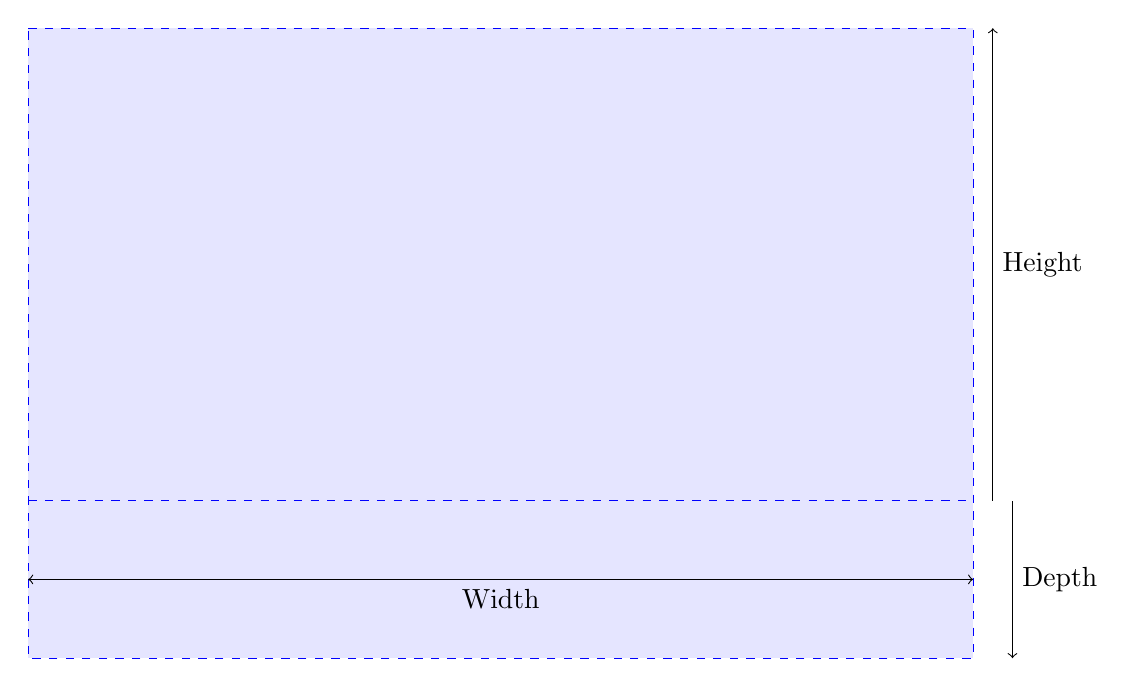
\begin{tikzpicture}[yscale=-1]
  \fill[blue!10] (0,-6) -- (12,-6) -- (12,2) -- (0,2) -- cycle;
  \draw[dashed,blue] (0,-6) -- (12,-6) -- (12,2) -- (0,2) -- cycle
  (0,0)--(12,0);

  \draw[<->] (0,1) -- (6,1) node[below]{Width} -- (12,1);

  \draw[<-] (12.25, -6) --
  (12.25,-3) node[right]{Height} -- (12.25,0);
  \draw[<-] (12.5, 2) --
  (12.5,1) node[right]{Depth} -- (12.5,0);
  \end{tikzpicture}
\caption{Box model for the {\tt mspace} element}
\label{fig:MspaceBoxModel}
\end{figure}

\subsubsection{String Literal {\tt <ms>}}

The MathML specification describes {\tt ms} as follows \cite{MathML3}:
%
\begin{quote}
The {\tt ms} element is used to represent "string literals" in expressions
meant to be interpreted by computer algebra systems or other systems containing
"programming languages".
\end{quote}

In general, {\tt ms} must be treated the same as the {\tt mtext}
element except that quotes are automatically added around its content.
The user agents may implement the {\tt lquote} or {\tt rquote} attributes
with the following style in the user agent stylesheet as suggested in section
\ref{UAStylesheet}:

\begin{lstlisting}
ms {
  display: inline;
}
ms:before, ms:after {
  content: "\0022"
}
ms[lquote]:before {
  content: attr(lquote)
}
ms[rquote]:after {
  content: attr(rquote)
}
\end{lstlisting}

\subsection{General Layout Schemata}

\subsubsection{Horizontally Group Sub-Expressions {\tt <mrow>}}\label{Mrow}

The MathML specification describes {\tt mrow} as follows \cite{MathML3}:
%
\begin{quote}
  An {\tt mrow} element is used to group together any number of sub-expressions,
  usually consisting of one or more {\tt mo} elements acting as "operators" on
  one or more other expressions that are their "operands".

  Several elements automatically treat their arguments as if they were
  contained in an {\tt mrow} element. See the discussion of inferred {\tt mrow}s
  in Section 3.1.3 Required Arguments. [...]

  {\tt mrow} elements are typically rendered visually as a horizontal row of
  their arguments, left to right in the order in which the arguments occur
  within a context with LTR directionality, or right to left within a context
  with RTL directionality. The {\tt dir} attribute can be used to specify the
  directionality for a specific mrow, otherwise it inherits the directionality
  from the context. [...] The description in Section 3.2.5 Operator, Fence,
  Separator or Accent {\tt <mo>} of suggested rendering rules for {\tt mo}
  elements assumes that all horizontal spacing between operators and their
  operands is added by the rendering of mo elements (or, more generally,
  embellished operators), not by the rendering of the {\tt mrow}s they are
  contained in.

  MathML provides support for both automatic and manual linebreaking of
  expressions (that is, to break excessively long expressions into several
  lines). All such linebreaks take place within mrows, whether they are
  explicitly marked up in the document, or inferred (See Section 3.1.3.1
  Inferred {\tt <mrow>}s), although the control of linebreaking is effected
  through attributes on other elements (See Section 3.1.7 Linebreaking of
  Expressions).
\end{quote}

The {\tt dir} attribute must be mapped to the {\tt direction} CSS property.
The current version of this document does not define any linebreaking algorithm
for the {\tt mrow} element, user agents may just ignore linebreaking rules.

User agents must follow the rules for inferred {\tt mrow}s described in
\cite{MathML3}. For example, to layout
{\tt <msqrt>child\_1 child\_2 child\_3 ...</msqrt>}, one must follow the layout
rules described for {\tt msqrt} in section \ref{radicals} using
the box of {\tt <mrow>child\_1 child\_2 child\_3 ... child\_N</mrow>} as the base.

The {\tt <mrow>child\_1 child\_2 child\_3 ... child\_N</mrow>} element is laid
out as show on figure \ref{fig:MrowBoxModel}. The boxes of $\text{child}_1$,
$\text{child}_2$, ... $\text{child}_N$ are put in a horizontal row
one after the other with all their baselines aligned. As a consequence of this
and of child box models, graphical elements such as fraction bars
or symmetric stretchy operators will also be
aligned along the math axis when the
{\tt AxisHeight\lxAddClass{MATH}} is unchanged (e.g. in the typical case
where the math font is unchanged).

As indicated in section \ref{LaTeX}, we generally do not add special spacing
around the children. For example, the leading and trailing spacing is already
included in the box metrics of embellished operators. The only exception is
for the italic correction: when a ``slanted'' child is
followed by a ``straight'' child, then an horizontal
space corresponding to the italic correction of the ``slanted'' child is added
between the two children \cite{OpenFontFormat3}. The italic correction of the
last child is also added after that child when it is ``slanted'' and when
the {\tt mrow} has more than one child. In this document, we interpret
``slanted'' as a child that is not an operator with
{\tt largeop="true"} (or an embellished operator whose {\tt mo} element core
has {\tt largeop="true"}) and has nonzero italic correction and ``straight''
as ``non-slanted''.

When the {\tt mrow} element contains only one child then the previous
description implies that the box metrics of the {\tt mrow} is the same as
the one of its unique child. As indicated in section \ref{BoxModel}, we thus
use the italic correction and top accent attachment of the child as the
corresponding values of the {\tt mrow} box.

\begin{figure}
\centering
  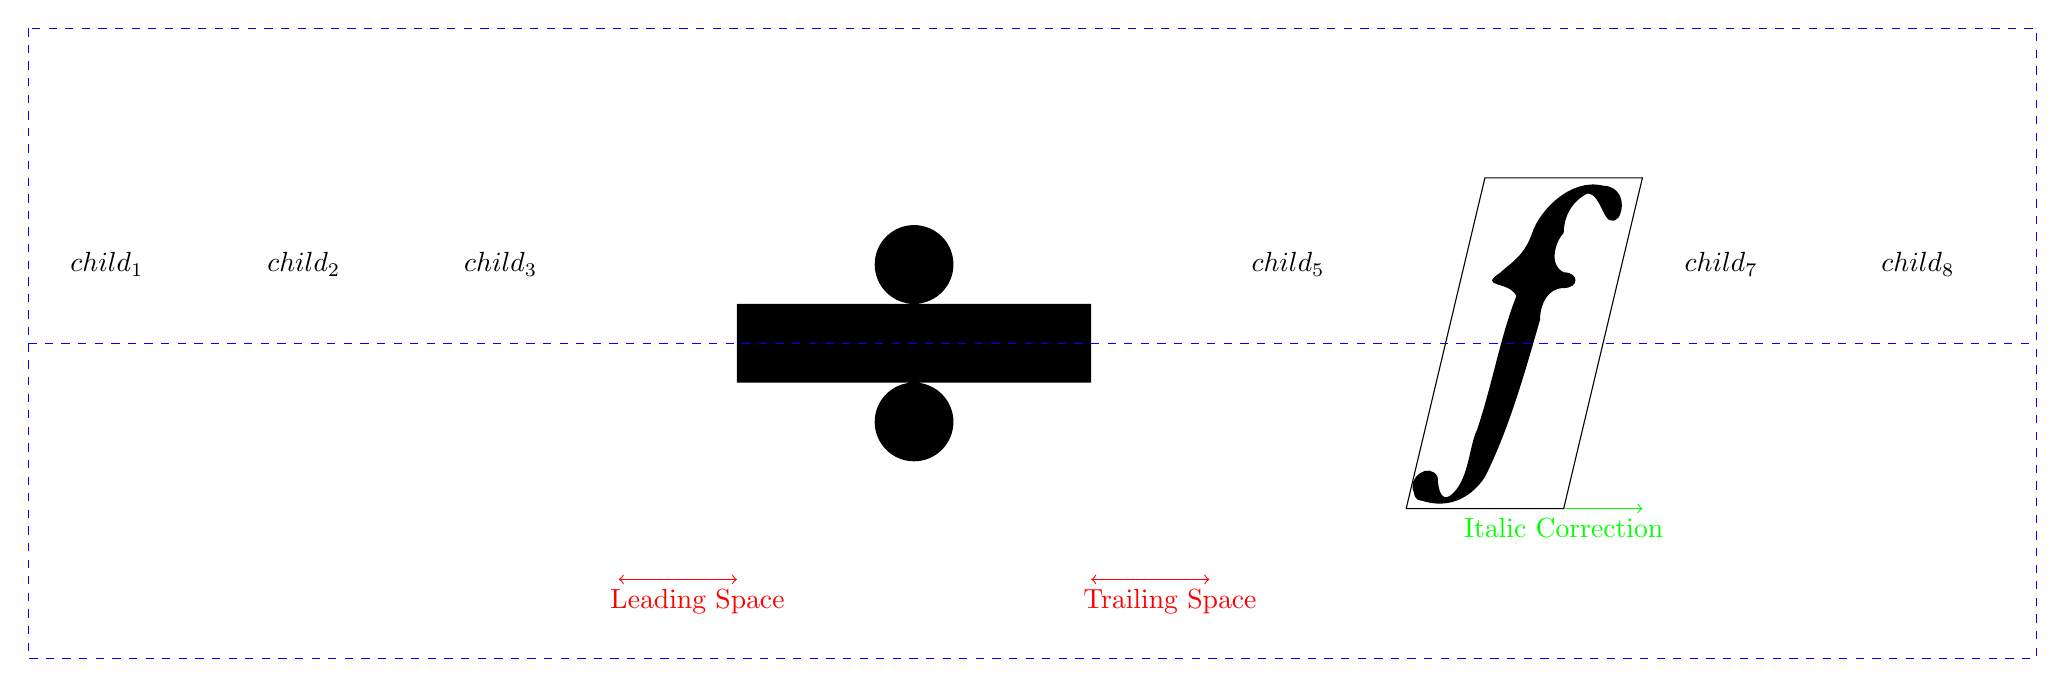
\begin{tikzpicture}[yscale=-1]
    \MathMLBox{0}{0}{.5}{1.5}{cyan}
    \draw(1,-1) node {$\text{child}_1$};

    \MathMLBox{2.5}{0}{.5}{1.2}{blue}
    \draw(3.5,-1) node {$\text{child}_2$};

    \MathMLBox{5}{0}{.5}{1.2}{cyan}
    \draw(6,-1) node {$\text{child}_3$};

    \MathMLBox{7.5}{0}{1.5}{1}{red}
    \fill[black] (9,-.5) rectangle (13.5,.5)
    (11.25,-1) circle (.5) (11.25,1) circle (.5);
    \draw[<->,red] (7.5,3) -- (8.5,3) node[below]{Leading Space} -- (9,3);
    \draw[<->,red] (13.5,3) -- (14.5,3) node[below]{Trailing Space} -- (15,3);

    \MathMLBox{15}{0}{.5}{1.4}{cyan}
    \draw(16,-1) node {$\text{child}_5$};

    \MathMLBox{17.5}{0}{.4}{1.35}{green}
    \begin{scope}[shift=({17.5,-2.1})]
    \begin{scope}[xscale=.1,yscale=.1]
    \fill[black] (1,40) .. controls (0,38) and (3,36) .. (4,38) .. controls (4,38) and (4,42) .. (6,40) .. controls (8,38) and (8,34) .. (9,32) .. controls (11,26) and (12,20) .. (14,15) .. controls (13,13) and (9,14) .. (12,12) .. controls (13,11) and (15,10) .. (16,7) .. controls (17,4) and (21,0) .. (25,1) .. controls (27,1) and (28,3) .. (27,5) .. controls (25,7) and (25,2) .. (23,2) .. controls (21,3) and (20,5) .. (20,7) .. controls (19,8) and (18,11) .. (20,12) .. controls (22,12) and (22,14) .. (20,14) .. controls (18,14) and (17,16) .. (17,18) .. controls (15,25) and (13,32) .. (10,38) .. controls (8,41) and (5,42) .. (2,41) .. controls (1,41) and (1,40) .. (1,40) -- cycle;
    \draw[black] (10,0) -- (30,0) -- (20,42) -- (0,42) -- cycle;
    \draw[green,->] (20,42) node[below]{Italic Correction} -- (30,42);
    \end{scope}
    \end{scope}

    \MathMLBox{20.5}{0}{.5}{1.1}{blue}
    \draw(21.5,-1) node {$\text{child}_7$};

    \MathMLBox{23}{0}{.5}{1.2}{cyan}
    \draw(24,-1) node {$\text{child}_8$};

    \draw[dashed,blue] (0,-4) rectangle (25.5,4) (0,0)--(25.5,0);
  \end{tikzpicture}
\caption{Box model for the {\tt mrow} element}
\label{fig:MrowBoxModel}
\end{figure}

\subsubsection{Fractions {\tt <mfrac>}}\label{Fractions}

The MathML specification describes {\tt mfrac} as follows \cite{MathML3}:
%
\begin{quote}
The {\tt mfrac} element is used for fractions. It can also be used to mark up
fraction-like objects such as binomial coefficients and Legendre symbols.
The syntax for {\tt mfrac} is

  {\tt <mfrac> numerator denominator </mfrac>}

The {\tt mfrac} element sets {\tt displaystyle} to {\tt "false"}, or if it was
already false increments {\tt scriptlevel} by 1, within numerator and
denominator.
\end{quote}

The {\tt displaystyle} and {\tt scriptlevel} changes be achieved with the
following style in the user agent stylesheet as suggested in section
\ref{UAStylesheet}:
%
\begin{lstlisting}
  mfrac > * {
    mathml-script-level: auto;
    mathml-math-style: inline;
  }
\end{lstlisting}
%

The axis of the {\tt mfrac} element is always given by
{\tt AxisHeight\lxAddClass{MATH}}.

The default line thickness is given by
{\tt FractionRuleThickness\lxAddClass{MATH}}
Use the {\tt linethickness} attribute \cite{MathML3} to determine the
actual thickness of the fraction bar. A percent or unitless length is
interpreted as a multiple of the default rule thickness and
the named values "thin", "medium" and "thick" are interpreted as
50\%, 100\%, 200\%.
The color and visibility of the fraction bar must honor the values given by the
{\tt color} and {\tt visibility} CSS properties on the {\tt mfrac} element.

If the actual line thickness is nonzero, the {\tt mfrac} element is laid out as
shown on figure \ref{fig:FractionBoxModel}.
The width is given by the maximum width of the
numerator and denominator and the numerator and denominator are horizontally
centered. A fraction bar with the actual thickness is drawn centered on the
axis height. The numerator and denominator are shifted
up and down using the values {\tt FractionNumeratorShiftUp\lxAddClass{MATH}},
{\tt FractionDenominatorShiftDown\lxAddClass{MATH}} in inline style and
{\tt FractionNumeratorDisplayStyleShiftUp\lxAddClass{MATH}},
{\tt FractionDenominatorDisplayStyleShiftDown\lxAddClass{MATH}}
in display style.
If necessary, these shift values are increased to ensure that the gaps between
the numerator/denominator and fraction bar satisfy the minimal values provided
by {\tt FractionDenominatorGapMin\lxAddClass{MATH}} and
{\tt FractionNumeratorGapMin\lxAddClass{MATH}} in inline style and
{\tt FractionDenominatorDisplayStyleGapMin\lxAddClass{MATH}} and
{\tt FractionNumeratorDisplayStyleGapMin\lxAddClass{MATH}}
in display style.

\begin{figure}
\centering
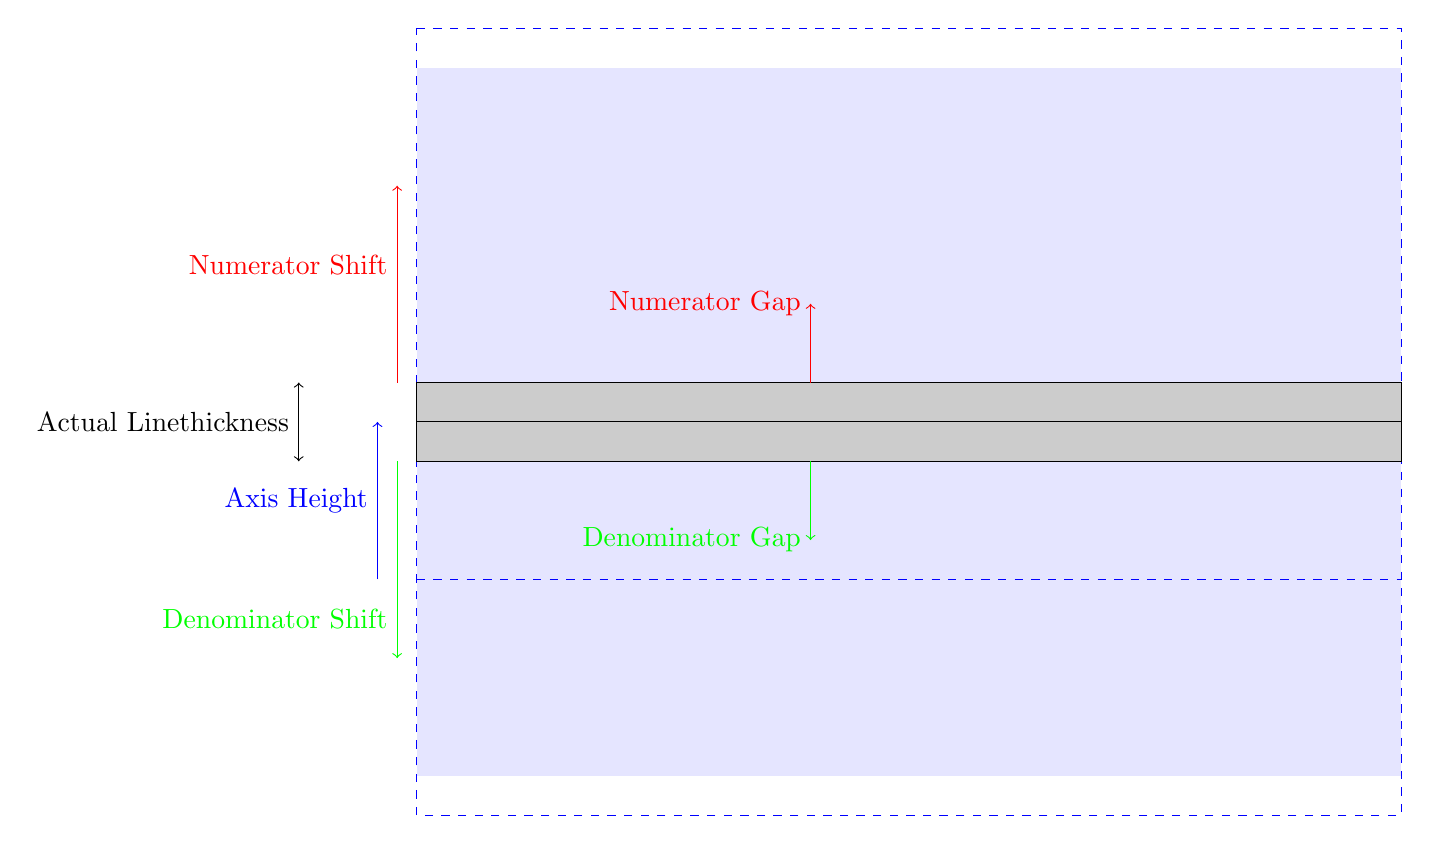
\begin{tikzpicture}[yscale=-1]
  \fill[blue!10] (0,-6.5) -- (12.5,-6.5) -- (12.5,2.5) -- (0,2.5) -- cycle;
  \MathMLBox{0}{-5}{2.5}{1}{red}
  \MathMLBox{3.75}{1}{1}{1}{green}
  \draw[dashed,blue] (0,-7) -- (12.5,-7) -- (12.5,3) -- (0,3) -- cycle
  (0,0) -- (12.5,0);
  \fill[black!20] (0,-2.5) -- (12.5,-2.5) -- (12.5,-1.5) -- (0,-1.5) -- cycle;
  \draw[black] (0,-2.5) -- (12.5,-2.5) -- (12.5,-1.5) -- (0,-1.5) -- cycle
  (0,-2) -- (12.5,-2);
  \draw[->,blue] (-.5,0) -- (-.5,-1) node[left]{Axis Height} -- (-.5,-2);
  \draw[<->,black] (-1.5,-2.5) --
  (-1.5,-2) node[left]{Actual Linethickness} -- (-1.5,-1.5);
  \draw[->,red] (-.25,-2.5) -- (-.25,-4)
  node[left]{Numerator Shift} -- (-.25,-5);
  \draw[->,green] (-.25,-1.5) -- (-.25,.5)
  node[left]{Denominator Shift} -- (-.25,1);
  \draw[->,red] (5,-2.5) -- (5,-3.5) node[left]{Numerator Gap};
  \draw[->,green] (5,-1.5) -- (5,-.5) node[left]{Denominator Gap};
\end{tikzpicture}
\caption{Box model for the {\tt mfrac} element}
\label{fig:FractionBoxModel}
\end{figure}

If the actual line thickness is zero,
the {\tt mfrac} element is instead laid out as
shown on figure \ref{fig:StackBoxModel}.
The gap between the top and bottom boxes
is equally split around the axis height. The relevant shift values are now
{\tt StackTopShiftUp\lxAddClass{MATH}},
{\tt StackBottomShiftDown\lxAddClass{MATH}} in inline style and
{\tt StackTopDisplayStyleShiftUp\lxAddClass{MATH}},
{\tt StackBottomDisplayStyleShiftDown\lxAddClass{MATH}} in display style.
If necessary, the two shift values are increased by a same value to ensure
the gap between the top and bottom boxes satisfy the values provided by
by {\tt StackGapMin\lxAddClass{MATH}} in inline style and
{\tt StackDisplayStyleGapMin\lxAddClass{MATH}} in display style.

\begin{figure}
\centering
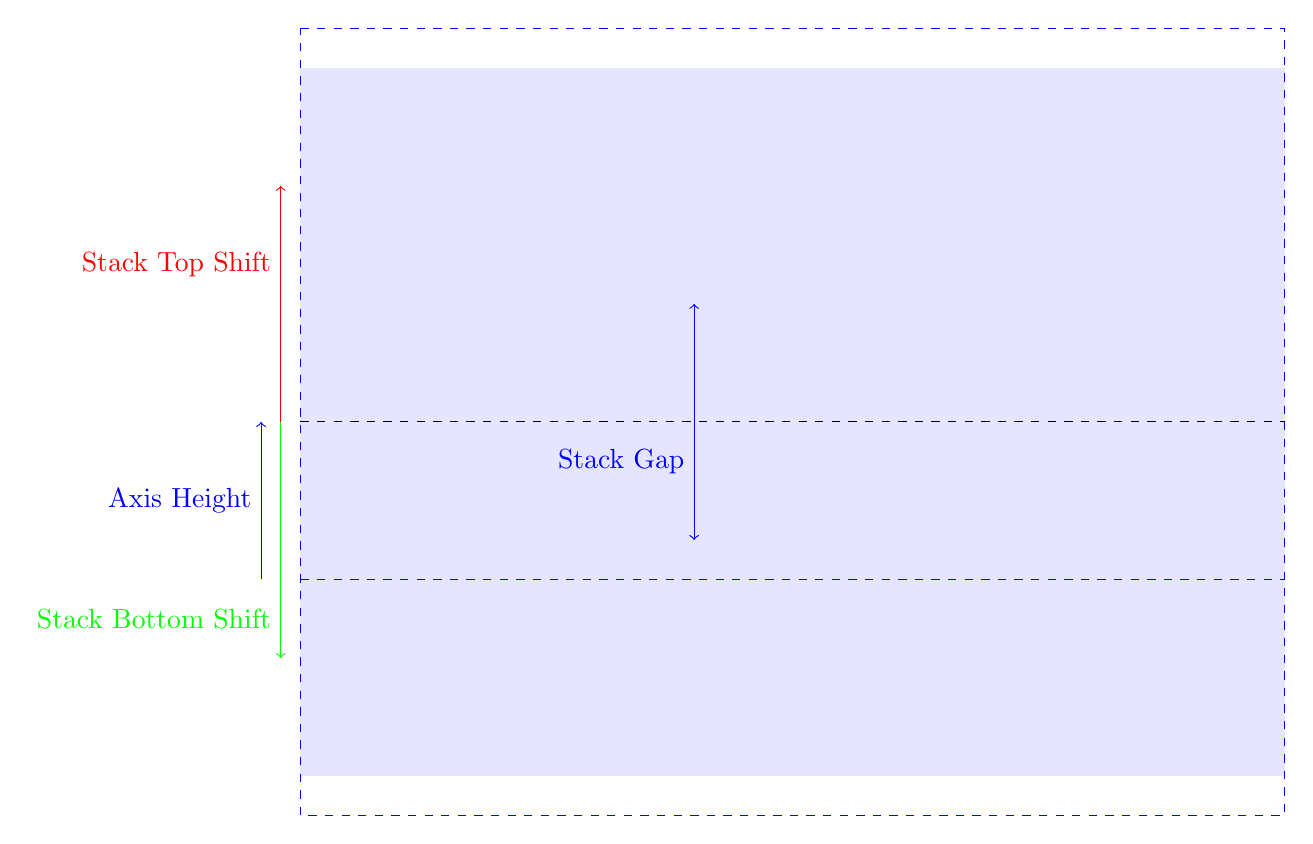
\begin{tikzpicture}[yscale=-1]
  \fill[blue!10] (0,-6.5) -- (12.5,-6.5) -- (12.5,2.5) -- (0,2.5) -- cycle;
  \MathMLBox{0}{-5}{2.5}{1}{red}
  \MathMLBox{3.75}{1}{1}{1}{green}
  \draw[dashed,blue] (0,-7) -- (12.5,-7) -- (12.5,3) -- (0,3) -- cycle
  (0,0) -- (12.5,0);
  \draw[black,dashed] (0,-2) -- (12.5,-2);
  \draw[->,blue] (-.5,0) -- (-.5,-1) node[left]{Axis Height} -- (-.5,-2);
  \draw[->,red] (-.25,-2) -- (-.25,-4)
  node[left]{Stack Top Shift} -- (-.25,-5);
  \draw[->,green] (-.25,-2) -- (-.25,.5)
  node[left]{Stack Bottom Shift} -- (-.25,1);
  \draw[<->,blue] (5,-3.5) -- (5,-1.5) node[left]{Stack Gap} --
  (5,-.5);
\end{tikzpicture}
\caption{Box model for the {\tt mfrac} element without bar}
\label{fig:StackBoxModel}
\end{figure}

If the numerator is an embellished operator and the {\tt mfrac} element is the
outermost element in this embellished operator hierarchy then the operator
leading and trailing spaces must be added around the fraction.

User agents may extend the box model to support the {\tt numalign},
{\tt denomalign} and {\tt bevelled} attributes \cite{MathML3}.

\subsubsection{Radicals {\tt <msqrt>}, {\tt <mroot>}}\label{radicals}

The MathML specification describes radicals as follows \cite{MathML3}:
%
\begin{quote}
These elements construct radicals. The {\tt msqrt} element is used for square
roots, while the {\tt mroot} element is used to draw radicals with indices,
e.g. a cube root. The syntax for these elements is:

{\tt
  <msqrt> base </msqrt> \\
  <mroot> base index </mroot>}

The {\tt mroot} element requires exactly 2 arguments. However, {\tt msqrt}
accepts a single argument, possibly being an inferred {\tt mrow} of multiple
children.

The {\tt mroot} element increments scriptlevel by 2, and sets displaystyle to
{\tt "false"},
within index, but leaves both attributes unchanged within base. The
{\tt msqrt} element leaves both attributes unchanged within its argument. [...]

Note that in a RTL directionality, the surd begins on the right, rather than
the left, along with the index in the case of mroot.
\end{quote}

The {\tt displaystyle} and {\tt scriptlevel} changes be achieved with the
following style in the user agent stylesheet as suggested in section
\ref{UAStylesheet}:
%
\begin{lstlisting}
  mroot > :not(:first-child) {
    mathml-script-level: increment 2;
    mathml-math-style: inline;
  }
\end{lstlisting}

The line thickness of the overbar is given by
{\tt RadicalRuleThickness\lxAddClass{MATH}}.
The gap between the overbar and base is given by
{\tt RadicalVerticalGap\lxAddClass{MATH}}
in inline style and {\tt RadicalDisplayStyleVerticalGap\lxAddClass{MATH}}
in display style.
The ascent above the overbase is given by {\tt RadicalExtraAscender\lxAddClass{MATH}}.
The surd is drawn by trying to vertically stretch the character
U+221A SQUARE ROOT
to at least the sum of the ink height of the base, the radical gap and the
radical rule thickness. If the CSS {\tt direction} is set to right-to-left,
then the surd is actually drawn from the glyph obtained by mirroring
U+221A SQUARE ROOT via the {\tt rtlm} OpenType feature.
The color and visibility of the surd and overbar must honor the values given by
the {\tt color} and {\tt visibility} CSS properties on the {\tt msqrt} element.

The {\tt msqrt} element is laid out as shown on figure
\ref{fig:SquareRootBoxModel}.
The width is given by the sum of the width of the surd and of the base.
The baseline of the square root matches the baseline of the base.
The ink box is determined from the ink boxes of the surd and base while the
logical box takes into account the extra ascender

\begin{figure}
\centering
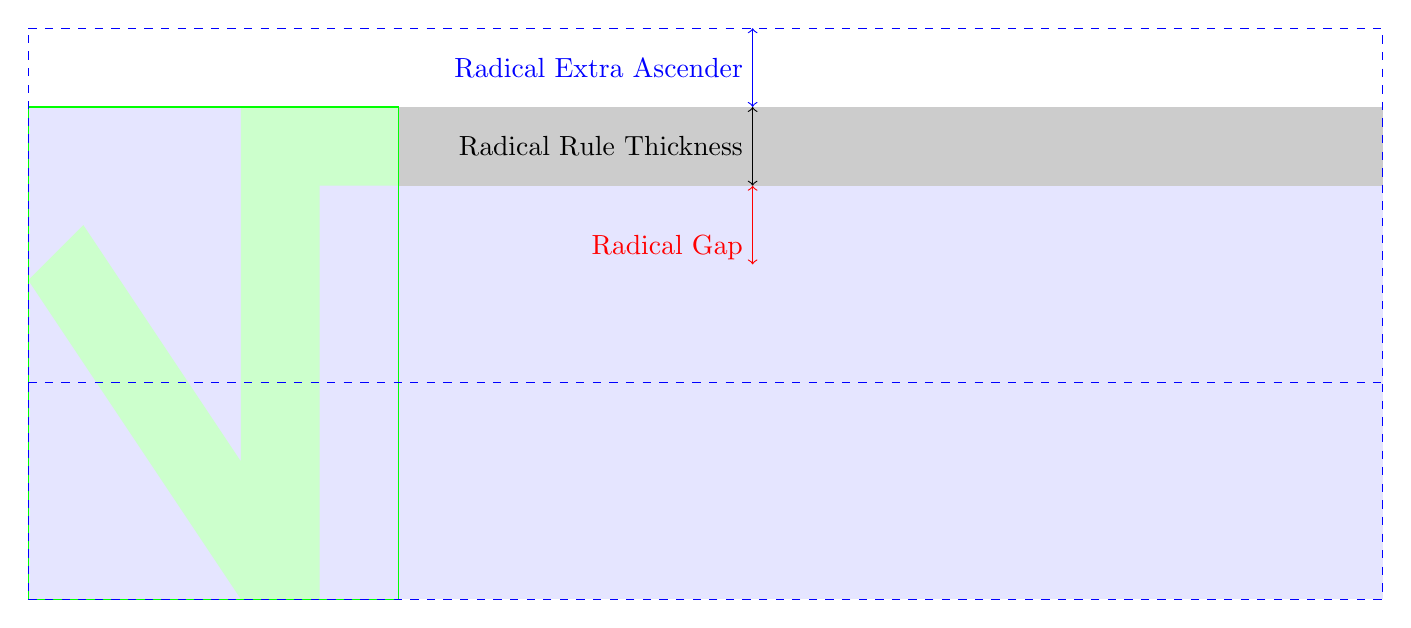
\begin{tikzpicture}[yscale=-1]
  \fill[blue!10] (-4.7,-2.5) -- (12.5,-2.5) --
  (12.5,3.75) -- (-4.7,3.75) -- cycle;

  \fill[black!20] (0,-2.5) -- (12.5,-2.5) -- (12.5,-1.5) -- (0,-1.5) -- cycle;

  \fill[green!20]
  (0,-2.5) -- (-2,-2.5) -- (-2,2) --
  (-4,-1) -- (-4.7,-.3) -- (-2.7,2.7) -- (-2,3.75) -- (-1,3.75) --
  (-1,-1.5) -- (0,-1.5) -- (0,-2.5);
  \draw[green] (-4.7,-2.5) -- (0,-2.5) -- (0,3.75) -- (-4.7,3.75) -- cycle;

  \MathMLBox{0}{1}{2.5}{1}{red}

  \draw[dashed,blue] (-4.7,-3.5) -- (12.5,-3.5) --
                     (12.5,3.75) -- (-4.7,3.75) -- cycle
                      (-4.7,1) -- (12.5,1);

  \draw[<->,blue] (4.5,-3.5) --
  (4.5,-3) node[left]{Radical Extra Ascender} -- (4.5,-2.5);

  \draw[<->,black] (4.5,-2.5) --
  (4.5,-2) node[left]{Radical Rule Thickness} -- (4.5,-1.5);

  \draw[<->,red] (4.5,-1.5) --
  (4.5,-1) node[below left]{Radical Gap} -- (4.5,-.5);
\end{tikzpicture}
\caption{Box model for the {\tt msqrt} element}
\label{fig:SquareRootBoxModel}
\end{figure}

The {\tt mroot} element is laid out as shown on figure \ref{fig:RootBoxModel}.
We start by ignoring the root index and we layout the base and surd as
shown on figure \ref{fig:SquareRootBoxModel} to obtain a box $B$.
The horizontal metrics of the {\tt mroot} element are obtained by putting
{\tt RadicalKernBeforeDegree\lxAddClass{MATH}}
before the root index, then placing the root index, then a kerning
of {\tt RadicalKernAfterDegree\lxAddClass{MATH}}
after the root index and finally placing $B$. In general
the kerning before the root index is positive while the kerning after it is
negative,
which means that the root element will have some space before it and that the
root index will overlap the surd.
For the vertical metrics of the {\tt mroot} element, we first take the baseline
of $B$ as the baseline. We graduate the ink height of $B$ with a linear
scale going from the bottom at coordinate 0 to the top at coordinate 1.
Then the baseline of the root index will
be vertically positioned at coordinate
{\tt RadicalDegreeBottomRaisePercent\lxAddClass{MATH}}.
Finally, we take into consideration the box of the root index and $B$ to deduce
the metrics for the whole box of the {\tt mroot} element.

\begin{figure}
\centering
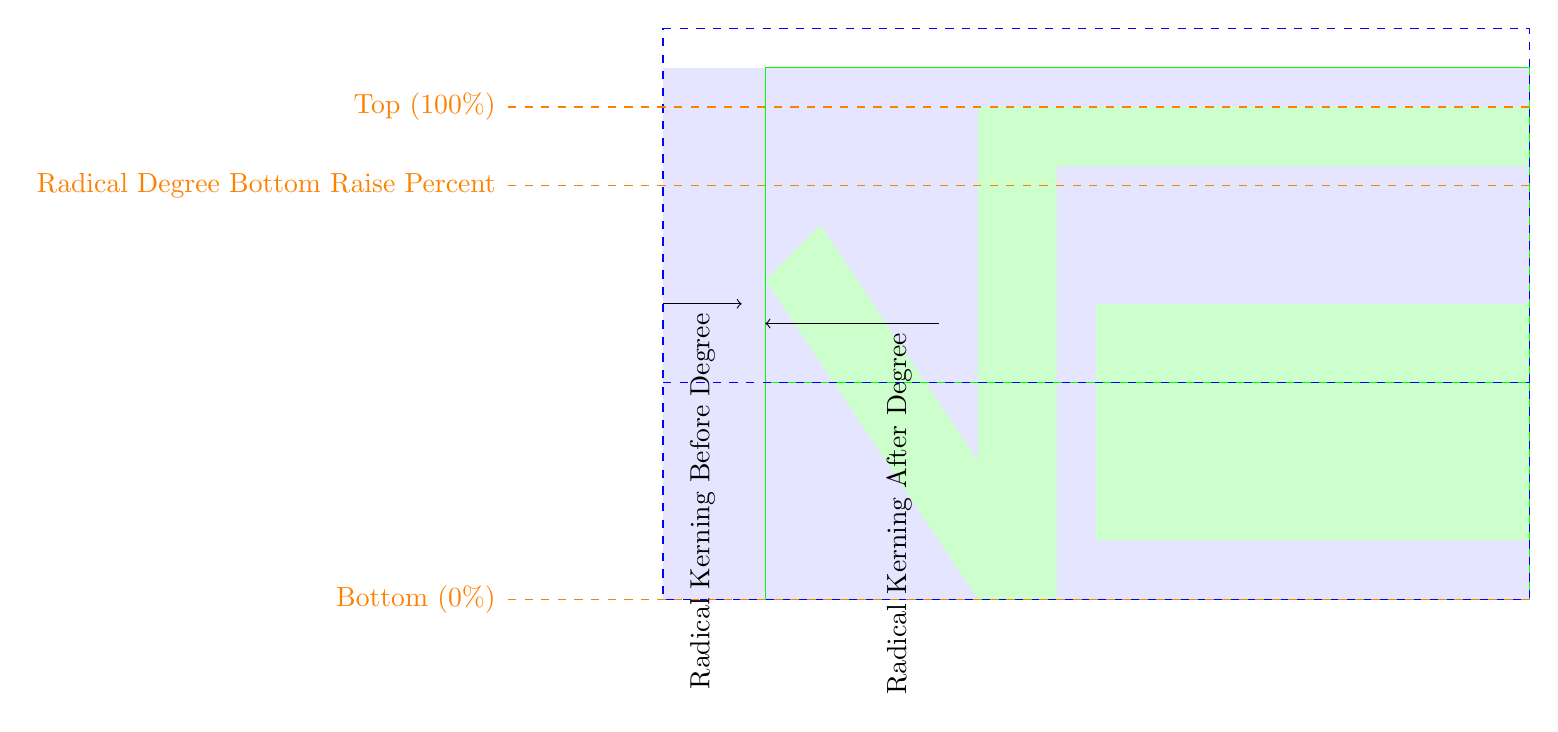
\begin{tikzpicture}[yscale=-1]
  \fill[blue!10] (0,-3) -- (11,-3) -- (11,3.75) -- (0,3.75) -- cycle;

  \begin{scope}[shift={(6,0)}]
  \fill[green!20]
  (5,-2.5) -- (-2,-2.5) -- (-2,2) --
  (-4,-1) -- (-4.7,-.3) -- (-2.7,2.7) -- (-2,3.75) -- (-1,3.75) --
  (-1,-1.75) -- (5,-1.75) -- (5,-2.5)
  (-.5,0) -- (5,0) -- (5,3) -- (-.5,3) -- cycle;
  \draw[green] (-4.7,-3) -- (5,-3) -- (5,3.75) -- (-4.7,3.75) -- cycle
  (-4.7,1)--(5,1);
  \end{scope}

  \MathMLBox{1}{-1.5}{.5}{1}{red}

  \draw[dashed,blue] (0,-3.5) -- (11,-3.5) -- (11,3.75) -- (0,3.75) -- cycle
  (0,1)--(11,1);

  \draw[dashed,orange](11,3.75)--(-2,3.75) node[left]{Bottom (0\%)};
  \draw[dashed,orange](11,-1.5)--(-2,-1.5) node[left]
       {Radical Degree Bottom Raise Percent};
  \draw[dashed,orange](11,-2.5)--(-2,-2.5) node[left]{Top (100\%)};

  \draw[->,black] (0,0) -- (.5,0) node[left,rotate=90]
       {Radical Kerning Before Degree} -- (1,0);
  \draw[->,black] (3.5,.25) -- (3,.25) node[left,rotate=90]
       {Radical Kerning After Degree} -- (1.3,.25);
\end{tikzpicture}
\caption{Box model for the {\tt mroot} element}
\label{fig:RootBoxModel}
\end{figure}

\subsubsection{Style Change {\tt <mstyle>}}

The MathML specification has a long description of {\tt mstyle} with several
ways to interpret the attributes, to handle inheritance and to deal with
additional exceptions. The most important points are \cite{MathML3}:
%
\begin{quote}
The {\tt mstyle} element is used to make style changes that affect the
rendering of its contents. [...]

The {\tt mstyle} element accepts a single argument, possibly being an inferred
{\tt mrow} of multiple children [...]

Loosely speaking, the effect of the {\tt mstyle} element is to change the
default value of an attribute for the elements it contains. Style changes work
in one of several ways, depending on the way in which default values are
specified for an attribute.
\end{quote}

For the layout algorithm described in this document, the
{\tt mstyle} element must be treated the same as the {\tt mrow} element.
However, some attributes on the {\tt mstyle} element must be mapped to CSS
properties as indicated in section \ref{CSSProperties}.
All the other {\tt mstyle}
attributes not defined in this document must be ignored.

\subsubsection{Error Message {\tt <merror>}}

The MathML specification describes {\tt merror} as follows \cite{MathML3}:
%
\begin{quote}
The {\tt merror} element displays its contents as an "error message". This
might be done, for example, by displaying the contents in red, flashing the
contents, or changing the background color. The contents can be any expression
or expression sequence.

{\tt merror} accepts a single argument possibly being an inferred {\tt mrow} of
multiple children. [...]
\end{quote}

For the layout algorithm described in this document, the
{\tt merror} element must be treated the same as the {\tt mrow} element.
The user agent stylesheet must set some CSS properties on the {\tt merror}
element in order to highlight the error.
As suggested in section \ref{UAStylesheet}, this can for example be achieved
with the rule:
%
\begin{lstlisting}
merror {
  outline: solid thin red;
  background-color: lightYellow;
}
\end{lstlisting}

\subsubsection{Adjust Space Around Content {\tt <mpadded>}}\label{mpadded}

The MathML specification describes {\tt mpadded} as follows \cite{MathML3}:
%
\begin{quote}
An {\tt mpadded} element renders the same as its child content, but with the
size of the child's bounding box and the relative positioning point of its
content modified according to {\tt mpadded}'s attributes. [...]

The {\tt mpadded} element accepts a single argument which may be an inferred
{\tt mrow} of multiple children
\end{quote}

See \cite{MathML3} for how the metrics of {\tt mpadded} element are determined.
Note that pseudo-units allows horizontal metrics to depend on vertical metrics,
for example {\tt width="2height"} which can be problematic to determine
intrinsic widths. Hence in the present document, if
the value of the {\tt width} and {\tt lspace} attributes contains
"height" or "depth" pseudo-units, then they must be ignored.

The {\tt mpadded} element is laid out as shown on figure
\ref{fig:MpaddedBoxModel}.
The height, depth and width of the content in \cite{MathML3} corresponds to
the logical box of the content. The content of the {\tt mpadded} element is
positioned from the origin of the {\tt mpadded} element as follows: We shift
the content
forward by a distance of {\tt lspace} and shift it upward by a distance of
{\tt voffset}. The logical metrics of the {\tt mpadded} element are given by the
height, depth and width of the {\tt mpadded} element described in
\cite{MathML3}. The ink metrics of the {\tt mpadded} element match their logical
metrics.

\begin{figure}
\centering
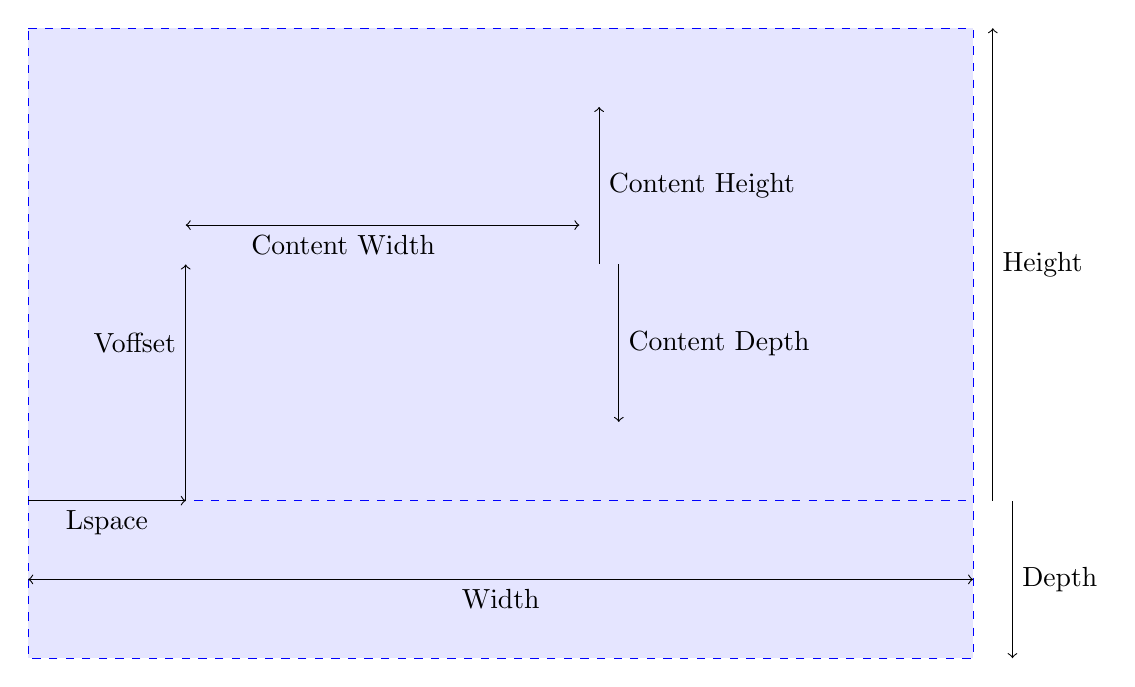
\begin{tikzpicture}[yscale=-1]
  \fill[blue!10] (0,-6) -- (12,-6) -- (12,2) -- (0,2) -- cycle;
  \draw[dashed,blue] (0,-6) -- (12,-6) -- (12,2) -- (0,2) -- cycle
  (0,0)--(12,0);

  \begin{scope}[shift={(2,-3)}]
    \MathMLBox{0}{0}{1}{1}{red}
    \draw[<->] (0,-.5) -- (2,-.5) node[below]{Content Width} -- (5,-.5);
    \draw[<-] (5.25, -2) --
    (5.25,-1) node[right]{Content Height} -- (5.25,0);
    \draw[<-] (5.5, 2) --
    (5.5,1) node[right]{Content Depth} -- (5.5,0);
  \end{scope}

  \draw[<->] (0,1) -- (6,1) node[below]{Width} -- (12,1);

  \draw[<-] (12.25, -6) --
  (12.25,-3) node[right]{Height} -- (12.25,0);
  \draw[<-] (12.5, 2) --
  (12.5,1) node[right]{Depth} -- (12.5,0);

  \draw[->] (0, 0) -- (1,0) node[below]{Lspace} -- (2,0);

  \draw[->] (2, 0) -- (2,-2) node[left]{Voffset} -- (2,-3);
\end{tikzpicture}
\caption{Box model for the {\tt mpadded} element}
\label{fig:MpaddedBoxModel}
\end{figure}

\subsubsection{Making Sub-Expressions Invisible {\tt <mphantom>}}

The MathML specification describes {\tt mphantom} as follows \cite{MathML3}:
%
\begin{quote}
The {\tt mphantom} element renders invisibly, but with the same size and other
dimensions, including baseline position, that its contents would have if they
were rendered normally. [...]

The {\tt mphantom} element accepts a single argument possibly being an inferred
{\tt mrow} of multiple children [...]
\end{quote}

For the layout algorithm described in this document, the
{\tt mphantom} element must be treated the same as the {\tt mrow} element.
The user agent stylesheet must set some CSS properties on the {\tt mphantom}
element in order to hide its content.
As suggested in section \ref{UAStylesheet}, this can for example be achieved
with the rule:
%
\begin{lstlisting}
mphantom {
  visibility: hidden;
}
\end{lstlisting}

\subsubsection{Expression Inside Pair of Fences {\tt <mfenced>}}

The MathML specification has a long description of {\tt mfenced} with several
exceptions for the parsing of its attributes. It gives a strict equivalence
between {\tt mfenced} and constructions that rely exclusively on {\tt mo} and
{\tt mrow} elements Here is the main point \cite{MathML3}:
%
\begin{quote}
The {\tt mfenced} element provides a convenient form in which to express common
constructs involving fences (i.e. braces, brackets, and parentheses),
possibly including separators (such as comma) between the arguments.
[...]
\end{quote}

This document does define any layout algorithm for the {\tt mfenced}
element. User agents may just treat them as equivalent to the {\tt mrow} element
or to an {\tt merror} element with a relevant error message indicating
unsupported markup.
Alternatively, {\tt mfenced} may be implemented using a shadow tree, anonymous
boxes, or any other methods that produce the same rendering as the equivalent
constructions with {\tt mo} and {\tt mrow} elements.

Authors are encouraged to use the equivalent constructions with {\tt mo} and
{\tt mrow} elements, instead of relying on the {\tt mfenced} element.

\subsubsection{Enclose Expression Inside Notation {\tt <menclose>}}\label{menclose}

The MathML specification describes {\tt menclose} as follows \cite{MathML3}:
%
\begin{quote}
The {\tt menclose} element renders its content inside the enclosing notation
specified by its notation attribute. {\tt menclose} accepts a single argument
possibly being an inferred {\tt mrow} of multiple children [...]
\end{quote}

The color and visibility of the {\tt menclose} notations must honor the values
given by the {\tt color} and {\tt visibility} CSS properties on the
{\tt menclose} element.

Based on \cite{OpenFontFormat3} \cite{TeXBook}, we use the notation $\xi_8$
from the TeXBook to denote the default rule thickness and use $3\xi_8$ for gaps.
We actually let $\xi_8$ be {\tt OverbarRuleThickness\lxAddClass{MATH}}.
Contrary to what is done in general, the $x$-axis direction of all notations
except {\tt radical} are independent of the CSS {\tt direction}.
In order to determine the metrics of the {\tt menclose} notation, we
compute each notation individually and take the union of the metrics:

\begin{enumerate}
\item The {\tt left} notation is drawn by putting a vertical bar of thickness
  $\xi_8$ on the left of the content of the {\tt menclose} element.
  The length of the bar is obtained by extending the height of the content
  with {\tt OverbarVerticalGap\lxAddClass{MATH}} plus
  {\tt OverbarRuleThickness\lxAddClass{MATH}} above
  and  {\tt UnderbarVerticalGap\lxAddClass{MATH}} plus
  {\tt UnderbarRuleThickness\lxAddClass{MATH}} below.
  The gap between the bar and the content is $3\xi_8$.
  The logical box is obtained by adding some space of width
  $\xi_8$ on the left of the bar. See figure \ref{fig:MencloseLeftBoxModel}.

  \begin{figure}
\centering
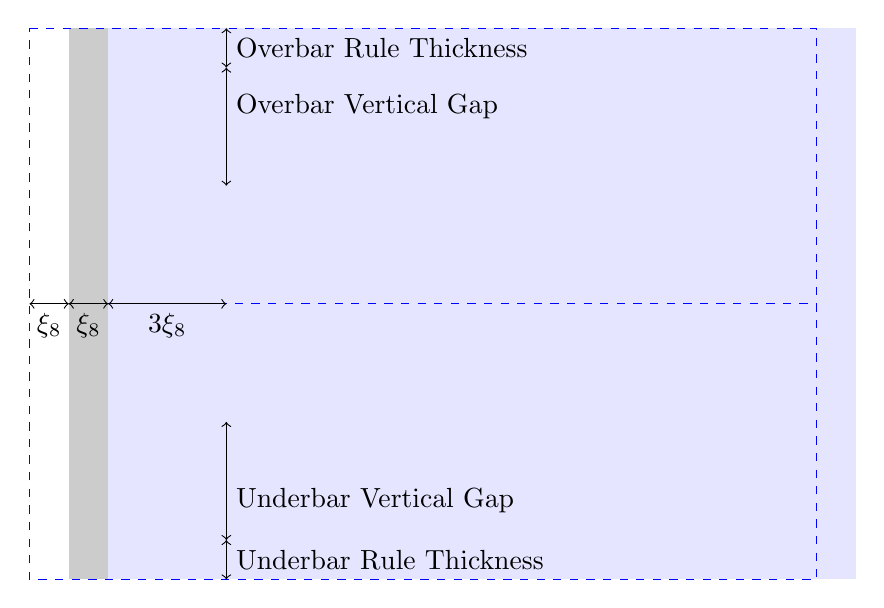
\begin{tikzpicture}[yscale=-1]

  \fill[blue!10] (0,-3.5) -- (10,-3.5) --
  (10,3.5) -- (0,3.5) -- cycle;
  \MathMLBox{2}{0}{1.5}{1}{red}

  \fill[black!20] (0,-3.5) -- (.5,-3.5) -- (.5,3.5) -- (0,3.5) -- cycle;

  \draw[dashed,blue](-.5,-3.5) -- (9.5,-3.5) -- (9.5,3.5) --
  (-.5,3.5) -- cycle (0,0) -- (9.5,0);

  \draw[<->] (2,-3) -- (2,-2.5) node[right]{Overbar Vertical Gap} -- (2,-1.5);
  \draw[<->] (2,-3) -- (2,-3.25)
    node[right]{Overbar Rule Thickness} -- (2,-3.5);

  \draw[<->] (.5,0) -- (1.25,0)node[below]{$3\xi_8$} -- (2,0);
  \draw[<->] (.5,0) -- (.25,0)node[below]{$\xi_8$} -- (0,0);
  \draw[<->] (-.5,0) -- (-.25,0)node[below]{$\xi_8$} -- (0,0);

  \draw[<->] (2,3) -- (2,2.5) node[right]{Underbar Vertical Gap} -- (2,1.5);
  \draw[<->] (2,3) -- (2,3.25)
    node[right]{Underbar Rule Thickness} -- (2,3.5);
\end{tikzpicture}
  \caption{Box model for the {\tt left}
    notation of the {\tt menclose} element}
\label{fig:MencloseLeftBoxModel}
\end{figure}

\item The {\tt right} notation is drawn the same as the {\tt left} notation,
  but with the vertical bar placed on the right.

\item The {\tt top} notation is drawn by putting an overbar of thickness
  {\tt OverbarRuleThickness\lxAddClass{MATH}}
  over the content of the {\tt menclose} element.
  The length of the bar is obtained by extending the width of the content
  with $4\xi_8$ on each side.
  The gap between the overbar and the content is
  {\tt OverbarVerticalGap\lxAddClass{MATH}}.
  The logical box is obtained by adding some space of height
  {\tt OverbarExtraAscender\lxAddClass{MATH}} above the bar.
  See figure \ref{fig:MencloseTopBoxModel}.

  \begin{figure}
\centering
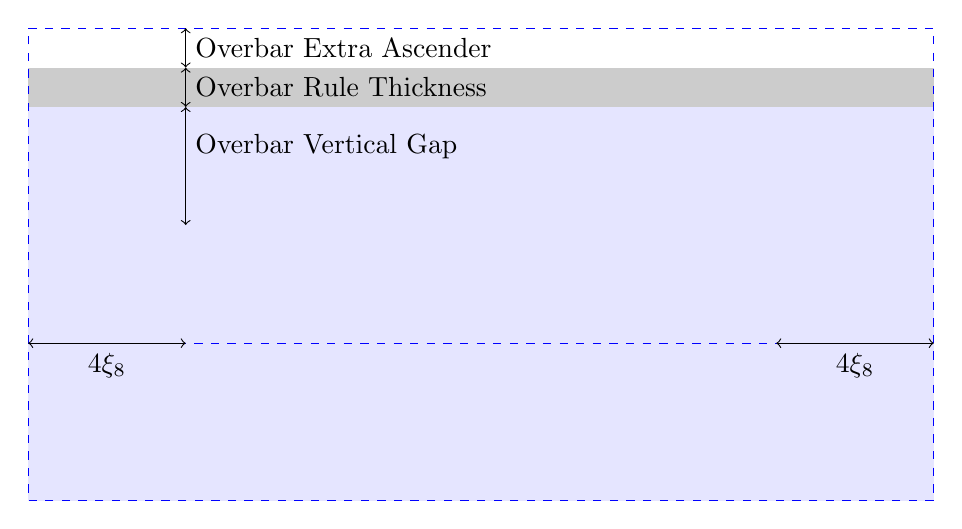
\begin{tikzpicture}[yscale=-1]

  \fill[blue!10] (0,-3.5) -- (11.5,-3.5) -- (11.5,2) -- (0,2) -- cycle;
  \MathMLBox{2}{0}{1.5}{1}{red}
  \fill[black!20] (0,-3.5) -- (11.5,-3.5) -- (11.5,-3) -- (0,-3) -- cycle;

  \draw[dashed,blue](0,-4) -- (11.5,-4) -- (11.5,2) -- (0,2) -- cycle
  (0,0) -- (11.5,0);

  \draw[<->] (2,-3) -- (2,-2.5) node[right]{Overbar Vertical Gap} -- (2,-1.5);
  \draw[<->] (2,-3) -- (2,-3.25)
    node[right]{Overbar Rule Thickness} -- (2,-3.5);
  \draw[<->] (2,-4) -- (2,-3.75)
    node[right]{Overbar Extra Ascender} -- (2,-3.5);

  \draw[<->] (0,0) -- (1,0)node[below]{$4\xi_8$} -- (2,0);
  \draw[<->] (9.5,0) -- (10.5,0)node[below]{$4\xi_8$} -- (11.5,0);
\end{tikzpicture}
  \caption{Box model for the {\tt roundedbox}
    notation of the {\tt top} element}
\label{fig:MencloseTopBoxModel}
\end{figure}

\item The {\tt bottom} notation is drawn the same as the {\tt top} notation,
  but with the vertical bar placed below the content and using parameters
  {\tt UnderbarRuleThickness\lxAddClass{MATH}},
  {\tt UnderbarVerticalGap\lxAddClass{MATH}}.
  and {\tt UnderExtraDescender\lxAddClass{MATH}}.

\item The {\tt box} notation is treated as equivalent to
  {\tt left right top bottom}.

\item To draw the {\tt roundedbox} notation, we consider the box
  obtained by expanding the ink box by $\frac{7\xi_8}{2}$ on each side.
  Using SVG terminology, we draw a rounded rectangle on this expanded box
  with parameters {\tt rx}, {\tt ry} and {\tt stroke-width} set to $\xi_8$
  \cite{SVG11}. To obtain the logical box we again add a space of $\xi_8$ on
  each side of the ink box. See figure \ref{fig:MencloseRoundedBoxBoxModel}.

  \begin{figure}
\centering
  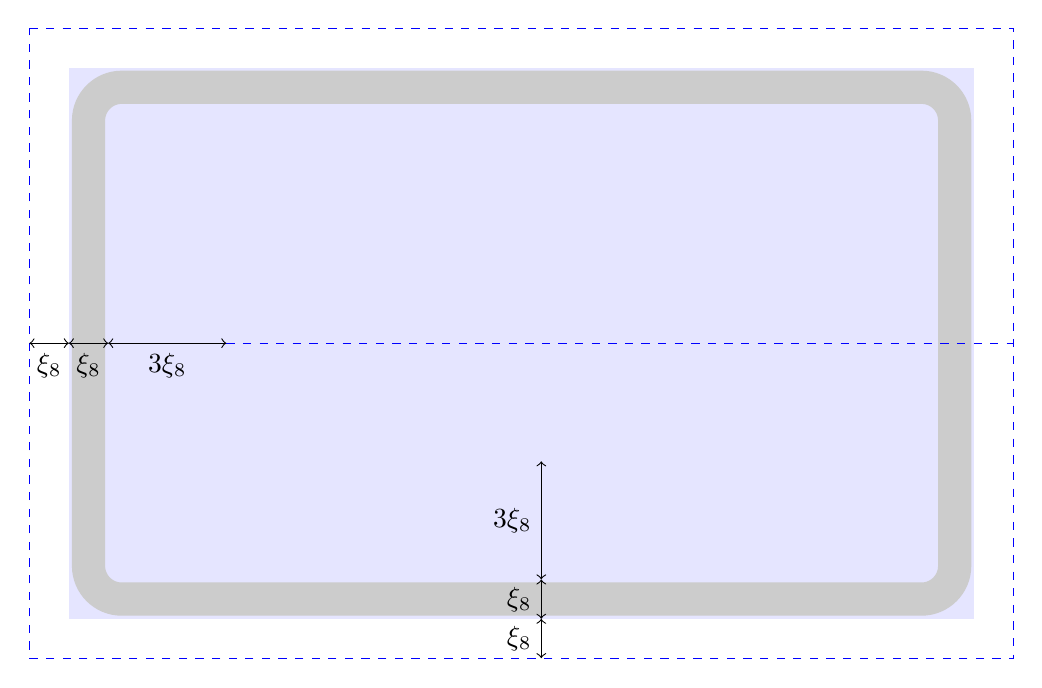
\begin{tikzpicture}[yscale=-1]

  \fill[blue!10]
  (-2,-3.5) -- (9.5,-3.5) -- (9.5,3.5) -- (-2,3.5) -- cycle;

  \MathMLBox{0}{0}{1.5}{1}{red};

  \draw[black!20,line width=12,rounded corners=12]
  (-1.75,-3.25) -- (9.25,-3.25) -- (9.25,3.25) -- (-1.75,3.25) -- cycle;

  \draw[dashed,blue]
  (-2.5,-4) -- (10,-4) -- (10,4) -- (-2.5,4) -- cycle
  (0,0) -- (10,0);

  \draw[<->] (0,0) -- (-.75,0)node[below]{$3\xi_8$} -- (-1.5,0);
  \draw[<->] (-1.5,0) -- (-1.75,0)node[below]{$\xi_8$} -- (-2,0);
  \draw[<->] (-2,0) -- (-2.25,0)node[below]{$\xi_8$} -- (-2.5,0);

  \draw[<->] (4,1.5) -- (4,2.25)node[left]{$3\xi_8$} -- (4,3);
  \draw[<->] (4,3.5) -- (4,3.25)node[left]{$\xi_8$} -- (4,3);
  \draw[<->] (4,3.5) -- (4,3.75)node[left]{$\xi_8$} -- (4,4);

\end{tikzpicture}
  \caption{Box model for the {\tt roundedbox}
    notation of the {\tt menclose} element}
\label{fig:MencloseRoundedBoxBoxModel}
\end{figure}

\item The {\tt actuarial} notation is treated as equivalent to {\tt right top}.

\item  The {\tt madruwb} notation is treated as equivalent to
  {\tt right bottom}.

\item The {\tt horizontalstrike} notation is drawn with an horizontal bar
  of thickness $\xi_8$ and
  vertically centered inside the {\tt menclose} content.
  This does not change the box metrics.
  See figure \ref{fig:MencloseHorizontalStrikeBoxModel}.

  \begin{figure}
\centering
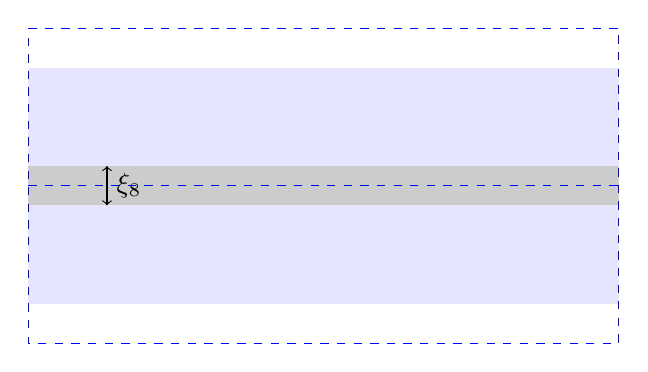
\begin{tikzpicture}[yscale=-1]

  \fill[blue!10] (0,-1.5) -- (7.5,-1.5) -- (7.5,1.5) -- (0,1.5) -- cycle;

  \MathMLBox{0}{0}{1.5}{1}{red};

  \fill[black!20] (0,-.25) -- (7.5,-.25) -- (7.5,.25) -- (0,.25) -- cycle;

  \draw[dashed,blue](0,-2) -- (7.5,-2) -- (7.5,2) -- (0,2) -- cycle
  (0,0) -- (7.5,0);

  \draw[<->] (1,-.25) -- (1,0) node[right]{$\xi_8$} -- (1,.25);
\end{tikzpicture}
  \caption{Box model for the {\tt horizontalstrike}
    notation of the {\tt menclose} element}
\label{fig:MencloseHorizontalStrikeBoxModel}
\end{figure}

\item The {\tt verticalstrike} notation is drawn the same as
  {\tt verticalstrike} but with a vertical bar
  of thickness $\xi_8$ and horizontally centered inside the {\tt menclose}
  content.
\item The {\tt updiagonalstrike} notation is drawn with a line
  of thickness $\xi_8$  going from the bottom left corner of the {\tt menclose}
  content to its top right corner. Using SVG terminology, the
  {\tt stroke-linecap} of the line is {\tt butt} \cite{SVG11}.
  As an approximation, the ink box
  is set equal to the logical box and obtained by increasing the original box
  from each side by $\frac{\xi_8}{2}$.
  See figure \ref{fig:MencloseUpDiagonalStrikeBoxModel}.

  \begin{figure}
\centering
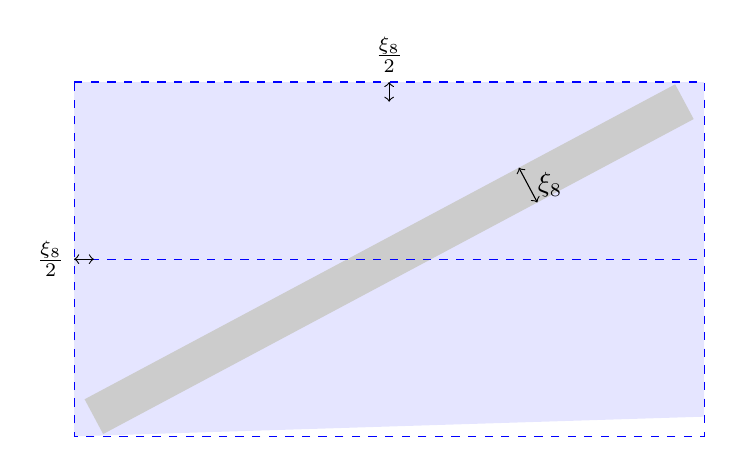
\begin{tikzpicture}[yscale=-1]
  \fill[blue!10]
     (-.25,-2.25) -- (7.75,-2.25) -- (7.75,2) -- (-.25,2.25) -- cycle;
  \MathMLBox{0}{0}{1.5}{1}{red};
  \begin{scope}[shift=({3.75,0}),rotate=-28.07248693585295]
  \fill[black!20] (-4.25,-.25) -- (4.25,-.25) --
                    (4.25,.25) -- (-4.25,.25) -- cycle;
  \draw[<->] (2,-.25) -- (2,0) node[right]{$\xi_8$} -- (2,.25);
  \end{scope}
  \draw[dashed,blue](-.25,-2.25) -- (7.75,-2.25) -- (7.75,2.25) -- (-.25,2.25)
  -- cycle (-.25,0) -- (7.75,0);

  \draw[<->] (0,0) -- (-.25,0) node[left]{$\frac{\xi_8}{2}$};
  \draw[<->] (3.75,-2) -- (3.75,-2.25) node[above]{$\frac{\xi_8}{2}$};
\end{tikzpicture}
  \caption{Box model for the {\tt updiagonalstrike}
    notation of the {\tt menclose} element}
\label{fig:MencloseUpDiagonalStrikeBoxModel}
\end{figure}

\item The {\tt downdiagonalstrike} notation is drawn as an
  {\tt updiagonalstrike}
  but the line strike goes from the top left corner to the bottom right corner.
  Using SVG terminology, the
  {\tt stroke-linecap} of the line is {\tt butt} \cite{SVG11}.
\item The {\tt radical} notation is drawn as described for {\tt msqrt}
  in section \ref{radicals}.
\item The {\tt longdiv} notation is drawn as {\tt radical} but independent
  of CSS {\tt direction}. U+221A SQUARE ROOT is replaced with
  U+0028 LEFT PARENTHESIS. The rule thickness is $\xi_8$,
  the gap between content and overbar is $3\xi_8$ and the extra ascender
  is $\xi_8$.
\item  To draw the {\tt circle} notation, we first consider the ink box of
  width $w$ and height $h$. We draw the ellipse
  of axes the axes of symmetry of this ink box, of radii
  $\frac{\sqrt{2}}{2} w$ and $\frac{\sqrt{2}}{2} h$ and of thickness $\xi_8$.
  We ensure that the logical box also has space $\xi_8$ around each side
  of the ellipse ink box.
  \begin{figure}
\centering
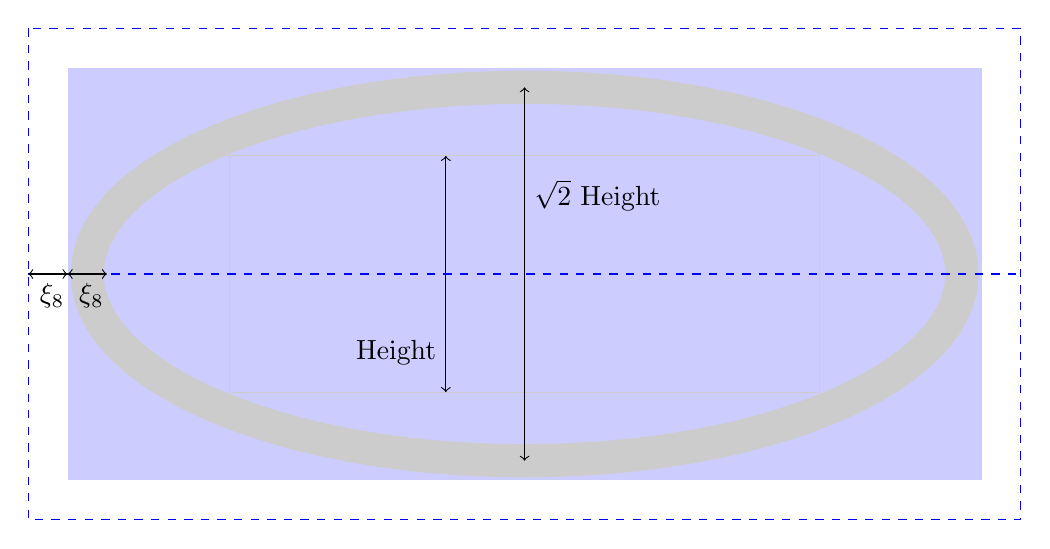
\begin{tikzpicture}[yscale=-1]

  \fill[blue!20]
  (-5.803300858899106,-2.621320343559643)
  rectangle (5.803300858899106,2.621320343559643);

  \MathMLBox{-3.75}{0}{1.5}{1}{red};

  \draw[black!20,line width=12]
  (0,0) ellipse (5.553300858899106 and 2.371320343559643);

  \draw[black!20]
  (-3.75,-1.5) rectangle (3.75,1.5);

  \draw[dashed,blue]
  (-6.303300858899106,-3.121320343559643)
  rectangle (6.303300858899106,3.121320343559643)
  (-6.303300858899106,0) -- (6.303300858899106,0);

  \draw[<->] (-6.303300858899106,0) --
  (-6,0)node[below]{$\xi_8$} --
  (-5.803300858899106,0);

  \draw[<->] (-5.803300858899106,0) --
  (-5.5,0)node[below]{$\xi_8$} --
  (-5.303300858899106,0);

  \draw[<->] (-1,-1.5) --
  (-1,1)node[left]{Height} --
  (-1,1.5);

  \draw[<->] (0,-2.371320343559643) --
  (0,-1)node[right]{$\sqrt{2}$ Height} --
  (0,2.371320343559643);

\end{tikzpicture}
  \caption{Box model for the {\tt circle}
    notation of the {\tt menclose} element}
\label{fig:MencloseCircleBoxModel}
\end{figure}

\item Other {\tt menclose} notations may be ignored.
\end{enumerate}

\subsection{Script and Limit Schemata}\label{ScriptAndLimitSchemata}

\subsubsection{Subscripts and Superscripts {\tt <msub>}, {\tt <msup>},
  {\tt <msubsup>}}\label{SubscriptsSuperscripts}

The MathML specification describes Subscripts and Superscripts as
follows \cite{MathML3}:
%
\begin{quote}
The msub element attaches a subscript to a base using the syntax

  {\tt <msub>} base subscript {\tt </msub>}

It increments {\tt scriptlevel} by 1, and sets {\tt displaystyle} to
{\tt "false"}, within subscript, but leaves both attributes unchanged within
base. [...]

The {\tt msup} element attaches a superscript to a base using the syntax

  {\tt <msup>} base superscript {\tt </msup>}

It increments {\tt scriptlevel} by 1, and sets {\tt displaystyle} to
{\tt "false"}, within superscript, but leaves both attributes unchanged within
base. [...]

The {\tt msubsup} element is used to attach both a subscript and superscript to
a base expression.

  {\tt <msubsup>} base subscript superscript {\tt </msubsup>}

It increments {\tt scriptlevel} by 1, and sets {\tt displaystyle} to
{\tt "false"}, within subscript and superscript, but leaves both attributes
unchanged within base. [...]
\end{quote}
%

As suggested in section section \ref{UAStylesheet}, the {\tt displaystyle} and
{\tt scriptlevel} changes be achieved with the
following style in the user agent stylesheet:
%
\begin{lstlisting}
msub > :not(:first-child),
msup > :not(:first-child),
msubsup > :not(:first-child) {
  mathml-script-level: increment 1;
  mathml-math-style: inline;
}
\end{lstlisting}
%

The {\tt msub} element is laid out as shown on figure \ref{fig:MsubBoxModel}.
The baseline is the baseline of the base while the baseline of the script is
shifted down by {\tt SubShift}, which is the minimal value honoring the
following conditions:
\begin{enumerate}
\item {\tt SubShift} is at least {\tt SubscriptShiftDown\lxAddClass{MATH}}.
\item The top of the subscript {\tt SubTop} with respect to the baseline
  is not above {\tt SubscriptTopMax\lxAddClass{MATH}}.
\item The drop {\tt SubscriptBaselineDrop} from the bottom of the base to
  the baseline of the script is at least
  {\tt SubscriptBaselineDropMin\lxAddClass{MATH}}.
\end{enumerate}

When determining
the logical box, a space of width {\tt SpaceAfterScript\lxAddClass{MATH}}
is added after
the subscript. By default, the leading edge of the subscript is aligned with
the trailing edge of the base. However, if the base is an operator with
{\tt largeop="true"} (or an embellished operator whose {\tt mo} element core
has {\tt largeop="true"}) the subscript is horizontally shifted backward
by the italic correction of the base.

\begin{figure}
\centering
  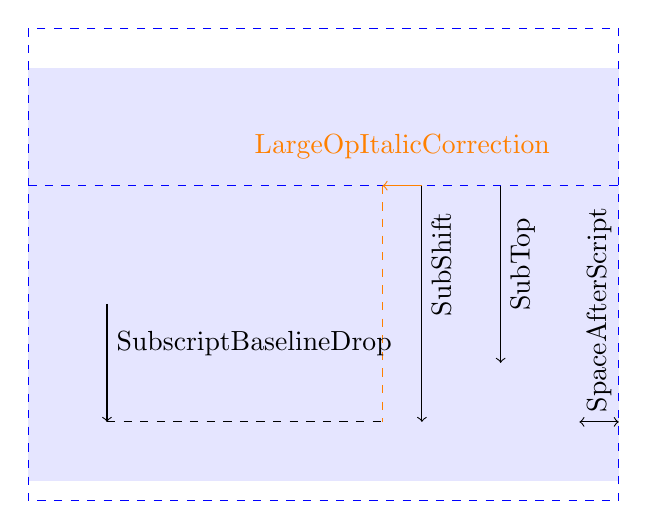
\begin{tikzpicture}[yscale=-1]

  \fill[blue!10](0,-1.5) rectangle (7.5,3.75);

  \MathMLBox{0}{0}{1}{1}{red};

  \MathMLBox{4.5}{3}{.5}{.5}{green};

  \draw[dashed,blue](0,-2) rectangle(7.5,4)
  (0,0)--(7.5,0);

   \draw[->] (5,0) -- (5,1)node[below,rotate=90]{SubShift} -- (5,3);

   \draw[orange,->] (5,0) -- (4.5,0);
   \draw[orange] (4.75, -.5) node{LargeOpItalicCorrection};
   \draw[dashed,orange] (4.5,0) -- (4.5,3);

   \draw[->] (6,0) -- (6,1)node[below,rotate=90]{SubTop} -- (6,2.25);

   \draw[<->] (7,3) -- (7.25,3)node[right,rotate=90]{SpaceAfterScript} -- (7.5,3);

   \draw[->] (1,1.5) -- (1,2)node[right]{SubscriptBaselineDrop} -- (1,3);
   \draw[dashed] (1,3) -- (4.5,3);
\end{tikzpicture}
\caption{Box model for the {\tt msub} element}
\label{fig:MsubBoxModel}
\end{figure}

The {\tt msup} element is laid out as shown on figure \ref{fig:MsupBoxModel}.
The baseline is the baseline of the base while the baseline of the script is
shifted up by {\tt SuperShift}, which is the minimal value honoring the
following conditions:
\begin{enumerate}
\item {\tt SubShift} is at least
  {\tt SuperscriptShiftUpCramped\lxAddClass{MATH}} if the {\tt msup} element is
  cramped (section \ref{LaTeX}) or at least
  {\tt SuperscriptShiftUp\lxAddClass{MATH}} otherwise.
\item The bottom of the superscript {\tt SuperBottom} with respect to the
  baseline is not below {\tt SuperscriptBottomMin\lxAddClass{MATH}}.
\item The drop {\tt SuperscriptBaselineDrop} from the top of the base to
  the baseline of the script is at most {\tt SuperscriptBaselineDropMax}.
\end{enumerate}

When determining
the logical box, a space of width {\tt SpaceAfterScript\lxAddClass{MATH}}
is added after
the superscript. By default, the leading edge of the superscript is aligned with
the trailing edge of the base and shifted forward by the italic correction
of the base, except if the base is an operator with
{\tt largeop="true"} (or an embellished operator whose {\tt mo} element core
has {\tt largeop="true"}).

\begin{figure}
\centering
  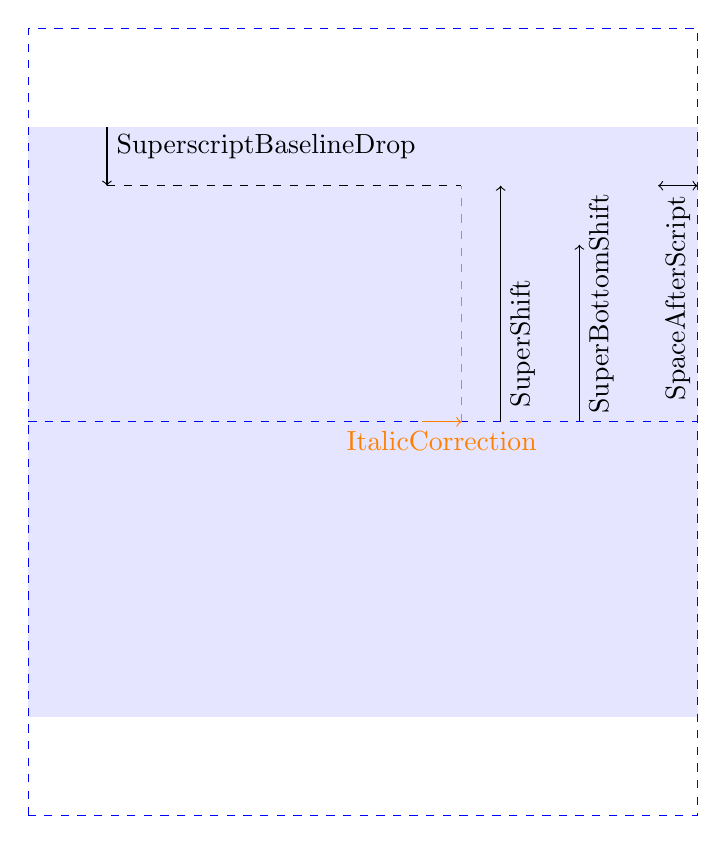
\begin{tikzpicture}[yscale=-1]

  \fill[blue!10](0,3.75) rectangle (8.5,-3.75);

  \MathMLBox{0}{0}{1}{2.5}{red};

  \MathMLBox{5.5}{-3}{.5}{.5}{green};

  \draw[dashed,blue](0,5) rectangle(8.5,-5)
  (0,0)--(8.5,0);

  \draw[->] (6,0) -- (6,-1)node[below,rotate=90]{SuperShift} -- (6,-3);

  \draw[orange,->] (5,0) --
   (5.25,0)node[below]{ItalicCorrection} -- (5.5,0);
  \draw[dashed,orange] (5.5,0)--(5.5,-3);

  \draw[->] (7,0) -- (7,-1.5)node[below,rotate=90]{SuperBottomShift} -- (7,-2.25);

  \draw[<->] (8,-3) -- (8.25,-3)node[left,rotate=90]{SpaceAfterScript} -- (8.5,-3);

  \draw[->] (1,-3.75) -- (1,-3.5)node[right]{SuperscriptBaselineDrop} -- (1,-3);
  \draw[dashed] (1,-3) -- (5.5,-3);
\end{tikzpicture}
\caption{Box model for the {\tt msup} element}
\label{fig:MsupBoxModel}
\end{figure}

The {\tt msubsup} element is laid out as shown on figure
\ref{fig:MsubsupBoxModel}.
The baseline is the baseline of the base while the baseline of the script is
shifted down by {\tt SubShift} and the superscript is shifted up by
{\tt SuperShift} which is initially set to the minimal values honoring the
following conditions:
\begin{enumerate}
\item {\tt SubShift} is at least
  {\tt SuperscriptShiftUpCramped\lxAddClass{MATH}} if the {\tt msup} element is
  cramped (section \ref{LaTeX}) or at least
  {\tt SuperscriptShiftUp\lxAddClass{MATH}} otherwise.
\item The top of the subscript {\tt SubTop} with respect to the baseline
  is not above {\tt SubscriptTopMax\lxAddClass{MATH}}.
\item The drop {\tt SuperscriptBaselineDrop} from the top of the base to
  the baseline of the script is at most {\tt SuperscriptBaselineDropMax}.
\item {\tt SubShift} is at least
  {\tt SuperscriptShiftUpCramped\lxAddClass{MATH}} if the {\tt msup} element is
  cramped (section \ref{LaTeX}) or at least
  {\tt SuperscriptShiftUp\lxAddClass{MATH}} otherwise.
\item The bottom of the superscript {\tt SuperBottom} with respect to the
  baseline is not below {\tt SuperscriptBottomMin\lxAddClass{MATH}}.
\item The drop {\tt SuperscriptBaselineDrop} from the top of the base to
  the baseline of the script is at most {\tt SuperscriptBaselineDropMax}.
\end{enumerate}

We then increase the gap {\tt SubSuperGap} between the bottom of the superscript
and the top of the subscript to ensure it is at least
{\tt SubSuperscriptGapMin\lxAddClass{MATH}}:
This is first done by continuing to shift the superscript up as long as the
{\tt SuperBottomShift} does not exceed
{\tt SuperscriptBottomMaxWithSubscript\lxAddClass{MATH}}
and next by continuing to shift the subscript down.

When determining
the logical box, a space of width {\tt SpaceAfterScript\lxAddClass{MATH}}
is added after
each script. By default the leading edges of the scripts are aligned with
the trailing edge and either the superscript is shifted forward by the italic
correction of the base. However, if the base is an operator with
{\tt largeop="true"} (or an embellished operator whose {\tt mo} element core
has {\tt largeop="true"}) then instead the subscript is shifted forward by the
italic correction of the base.

\begin{figure}
\centering
  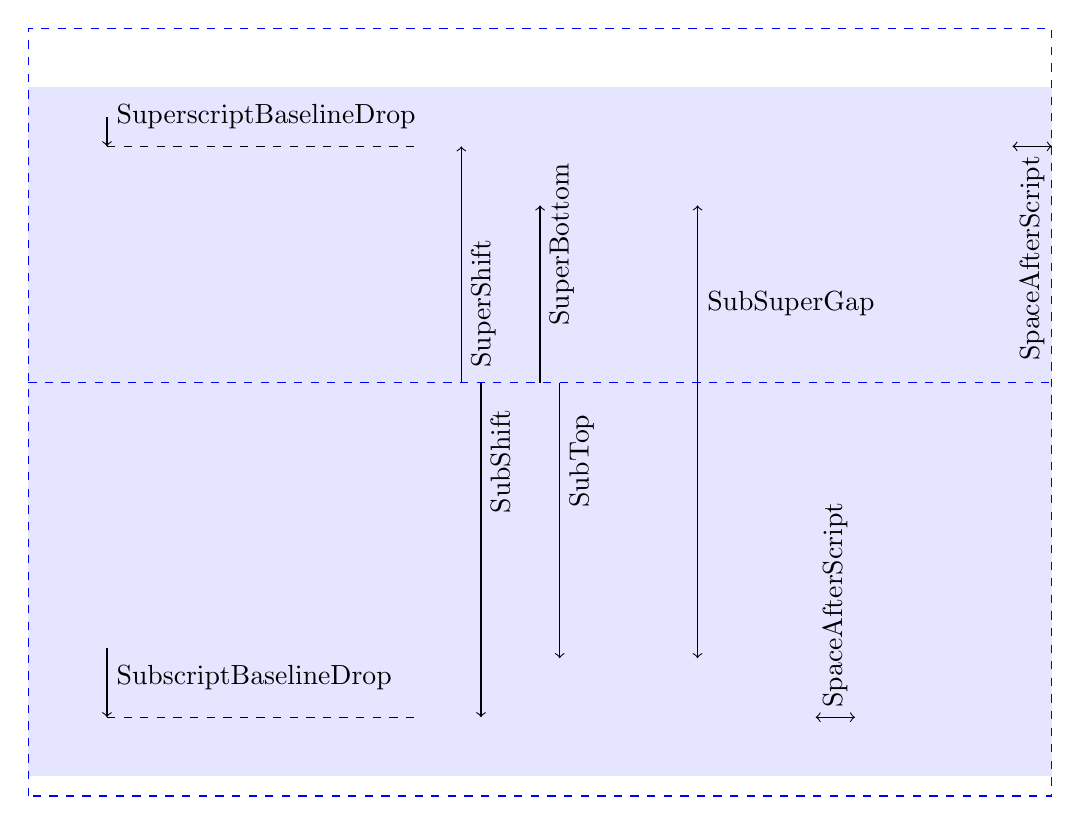
\begin{tikzpicture}[yscale=-1]

  \fill[blue!10](0,5) rectangle (13,-3.75);

  \MathMLBox{0}{0}{1}{2.25}{red};

  \MathMLBox{5}{-3}{1.5}{.5}{green};

  \draw[dashed,blue](0,5.25) rectangle(13,-4.5)
  (0,0)--(13,0);

  \draw[->] (5.5,0) -- (5.5,-1)node[below,rotate=90]{SuperShift} -- (5.5,-3);

  \draw[->] (6.5,0) -- (6.5,-1.75)node[below,rotate=90]{SuperBottom} -- (6.5,-2.25);

  \draw[<->] (12.5,-3) -- (12.75,-3)node[left,rotate=90]{SpaceAfterScript} -- (13,-3);

  \MathMLBox{5}{4.25}{1}{.5}{green};

   \draw[->] (5.75,0) -- (5.75,1)node[below,rotate=90]{SubShift} -- (5.75,4.25);

  \draw[->] (6.75,0) -- (6.75,1)node[below,rotate=90]{SubTop} -- (6.75,3.5);

  \draw[<->] (10,4.25) -- (10.25,4.25)node[right,rotate=90]{SpaceAfterScript} -- (10.5,4.25);

   \draw[<->] (8.5,-2.25) -- (8.5,-1)node[right]{SubSuperGap} -- (8.5,3.5);

   \draw[->] (1,-3.375) node[right]{SuperscriptBaselineDrop} -- (1,-3);
   \draw[dashed] (1,-3) -- (5,-3);

   \draw[->] (1,3.375) -- (1,3.75) node[right]{SubscriptBaselineDrop} -- (1,4.25);
   \draw[dashed] (1,4.25) -- (5,4.25);
\end{tikzpicture}
\caption{Box model for the {\tt msubsup} element}
\label{fig:MsubsupBoxModel}
\end{figure}

User Agents may ignore the attributes {\tt subscriptshift} and
{\tt superscriptshift} or may interpret them as minimal values
to satisfy when determining {\tt SubShift} and {\tt SuperShift} respectively.

\subsubsection{Underscripts and Overscripts  {\tt <munder>}, {\tt <mover>},
  {\tt <munderover>}}\label{UnderscriptsOverscripts}

The MathML specification describes Underscripts and Overscripts as
follows \cite{MathML3}:
%
\begin{quote}
The {\tt munder} element attaches an accent or limit placed under a base using
the syntax

  {\tt <munder>} base underscript {\tt </munder>}

It always sets {\tt displaystyle} to {\tt "false"} within the underscript, but
increments {\tt scriptlevel} by 1 only when {\tt accentunder} is
{\tt "false"}. Within base, it always leaves both attributes unchanged.[...]

If base is an operator with {\tt movablelimits="true"} (or an embellished
operator whose {\tt mo} element core has {\tt movablelimits="true"}), and
{\tt displaystyle="false"}, then underscript is drawn in a subscript position.
In this case, the {\tt accentunder} attribute is ignored. [...]

The {\tt mover} element attaches an accent or limit placed over a base using
the syntax

  {\tt <mover> base overscript </mover>}

It always sets {\tt displaystyle} to {\tt "false"} within overscript, but
increments {\tt scriptlevel} by 1 only when accent is {\tt "false"}.
Within base, it
always leaves both attributes unchanged.[...]

If base is an operator with {\tt movablelimits="true"} (or an embellished
operator whose {\tt mo} element core has {\tt movablelimits="true"}), and
{\tt displaystyle="false"}, then overscript is drawn in a superscript position.
In this case, the {\tt accent} attribute is ignored.[...]

The {\tt munderover} element attaches accents or limits placed both over and
under a base using the syntax

  {\tt <munderover> base underscript overscript </munderover>}

It always sets {\tt displaystyle} to {\tt "false"} within underscript and
overscript, but increments {\tt scriptlevel} by 1 only when {\tt accentunder}
or {\tt accent}, respectively, are {\tt "false"}. Within base, it always leaves
both attributes unchanged. [...]

If base is an operator with {\tt movablelimits="true"} (or an embellished
operator whose {\tt mo} element core has {\tt movablelimits="true"}), and
{\tt displaystyle="false"}, then underscript and overscript are drawn in a
subscript and superscript position, respectively. In this case, the
{\tt accentunder} and {\tt accent} attributes are ignored. [...]
\end{quote}
%

User Agents must perform the {\tt scriptlevel} increment by checking
the appropriate {\tt accent} or {\tt accentunder} value, which can not be done
using only CSS. However, {\tt displaystyle} changes can be achieved with the
following style in the user agent stylesheet, as suggested in section
\ref{UAStylesheet}:
%
\begin{lstlisting}
munder > :not(:first-child),
mover > :not(:first-child),
munderover > :not(:first-child) {
  mathml-math-style: inline;
}
\end{lstlisting}
%

In cases where underscript and overscript are drawn as subscript and
superscript position then the layout algorithm is the same as section
\ref{SubscriptsSuperscripts}. Note that in that case,
{\tt accent} or {\tt accentunder} are ignored so the scriptlevel increment is
always performed.

The general layout of {\tt munderover} is shown on figure
\ref{fig:MunderoverBoxModel}.
The overscript is placed above the base, the underscript below the base
and by default are aligned with respect to their geometrical center.
If the overscript is an accent and has a {\tt TopAccentAttachment}
value, then this value may be used to horizontally align the accent instead
of its geometrical center.
{\tt OverShift} is the distance between the top ink
of the base and the baseline of the overscript, {\tt OverGap} is the distance
between the top ink of the base and the bottom ink of the overscript,
{\tt OverExtraAscender} is extra space to add above the overscript when
determining the logical box. {\tt UnderShift}, {\tt UnderGap} and
{\tt UnderExtraAscender} are defined similarly for the underscripts.
We distinguish three cases:

\begin{enumerate}
\item If the base is an operator with {\tt largeop="true"}
  (or an embellished operator whose {\tt mo} element core has
  {\tt largeop="true"}) then ensure that {\tt OverGap} is at least
  {\tt UpperLimitGapMin\lxAddClass{MATH}}, that {\tt OverShift} is at least
  {\tt UpperLimitBaselineRiseMin\lxAddClass{MATH}} that {\tt UnderGap} is at
  least
  {\tt LowerLimitGapMin\lxAddClass{MATH}}, that {\tt UnderShift} is at least
  {\tt LowerLimitBaselineDropMin\lxAddClass{MATH}}.
  {\tt OverExtraAscender} and
  {\tt UnderExtraAscender} are zero. The
  underscript is shifted backward by half the italic correction of the base.
  The overscript is shifted forward by half the italic correction of the base.
\item If the base is an operator with {\tt stretchy="true"}
  (or an embellished operator whose {\tt mo} element core has
  {\tt stretchy="true"}). Then ensure that {\tt OverGap} is at least
  {\tt StretchStackGapBelowMin\lxAddClass{MATH}}, that {\tt OverShift} is at
  least
  {\tt StretchStackTopShiftUp\lxAddClass{MATH}} that {\tt UnderGap} is at least
  {\tt StretchStackGapAboveMin\lxAddClass{MATH}},
  that {\tt UnderShift} is at least
  {\tt StretchStackBottomShiftDown\lxAddClass{MATH}}.
  {\tt OverExtraAscender} and
  {\tt UnderExtraAscender} are zero.
\item In other cases we proceed as follows.
  We first ensure that {\tt UnderGap} is at least
  {\tt UnderbarVerticalGap\lxAddClass{MATH}}.
  If overscript is an accent
  and the ink ascent of the base does not exceed
  {\tt AccentBaseHeight\lxAddClass{MATH}}
  then we just align the baseline of the overscript with the baseline
  of the base. Otherwise, we ensure that {\tt OverGap} is at least
  {\tt OverbarVerticalGap\lxAddClass{MATH}}. Finally,
  {\tt OverExtraAscender} and
  {\tt OverExtraAscender} are respectively set to
  {\tt OverbarExtraAscender\lxAddClass{MATH}}
  and {\tt UnderExtraAscender\lxAddClass{MATH}}.
\end{enumerate}

\begin{figure}
\centering
  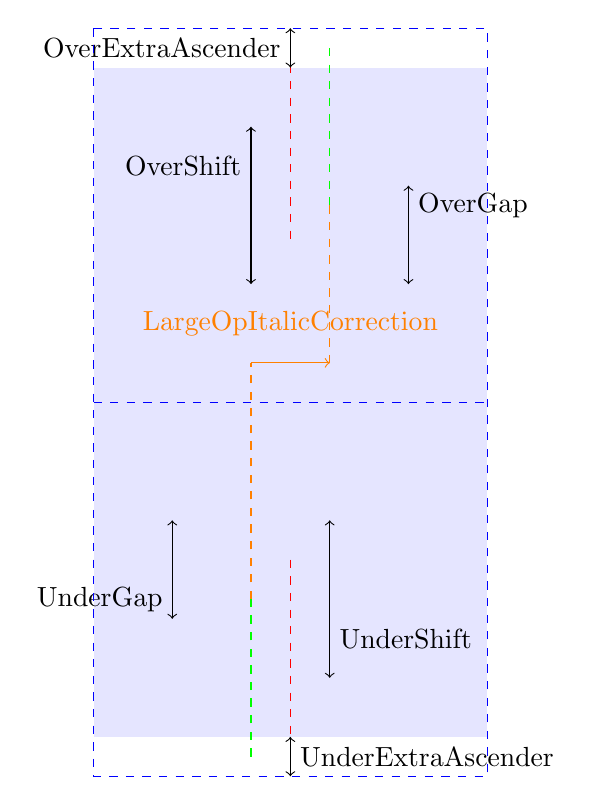
\begin{tikzpicture}[yscale=-1]

  \fill[blue!10](0,-4.25) rectangle (5,4.25);

  \MathMLBox{0.75}{3.5}{.5}{.5}{green};
  \draw[green,dashed](2,4.5)--(2,2.5);

  \MathMLBox{1.75}{-3.5}{.5}{.5}{green};
  \draw[green,dashed](3,-4.5)--(3,-2.5);

  \MathMLBox{0}{0}{1}{1}{red};
  \draw[red,dashed](2.5,-4.5)--(2.5,-2) (2.5,2)--(2.5,4.5);

  \draw[<->] (4,-1.5) -- (4,-2.5)node[right]{OverGap} -- (4,-2.75);
  \draw[<->] (2,-1.5) -- (2,-3)node[left]{OverShift} -- (2,-3.5);
  \draw[<->] (2.5,-4.25) --
             (2.5,-4.5)node[left]{OverExtraAscender} -- (2.5,-4.75);

  \draw[<->] (1,1.5) -- (1,2.5)node[left]{UnderGap} -- (1,2.75);
  \draw[<->] (3,1.5) -- (3,3)node[right]{UnderShift} -- (3,3.5);
  \draw[<->] (2.5,4.25) --
             (2.5,4.5)node[right]{UnderExtraAscender} -- (2.5,4.75);

  \draw[dashed,blue](0,-4.75) rectangle (5,4.75)
  (0,0)--(5,0);

  \draw[orange,->] (2,-.5) -- (3,-.5);
  \draw[orange] (2.5,-1)node{LargeOpItalicCorrection} ;
  \draw[orange,dashed](2,2.5) -- (2,-.5) (3,-2.5) --(3,-.5);

\end{tikzpicture}
\caption{Box model for the {\tt munderover} element}
\label{fig:MunderoverBoxModel}
\end{figure}

The layout of {\tt munder} and {\tt mover} is the same as the one of
{\tt munderover} except that one script and its corresponding extra space
are ignored.

User Agents may ignore the {\tt align} attribute. Alternatively, when it
is either {\tt left} or {\tt right}, then it may be used to the
alignment of the base, underscript and overscript along the specified edge.
Note that these values are independent of CSS {\tt direction}.

\subsubsection{Prescripts and Tensor Indices \tt <mmultiscripts>}

The MathML specification describes the {\tt mmultiscripts} element as
follows \cite{MathML3}:
%
\begin{quote}
Presubscripts and tensor notations are represented by a single element,
{\tt mmultiscripts}, using the syntax:

{\tt <mmultiscripts> \\
  base \\
  (subscript superscript)* \\
  {[} <mprescripts/> (presubscript presuperscript)* {]} \\
</mmultiscripts>}

This element allows the representation of any number of vertically-aligned
pairs of subscripts and superscripts, attached to one base expression. It
supports both postscripts and prescripts. Missing scripts can be represented
by the empty element {\tt none}.

{[}...{]}

The {\tt mmultiscripts} element increments {\tt scriptlevel} by 1, and sets
{\tt displaystyle} to {\tt "false"}, within each of its arguments except base,
but leaves both attributes unchanged within base. [...]
\end{quote}
%

The {\tt displaystyle} and {\tt scriptlevel} changes be achieved with the
following style in the user agent stylesheet as suggested in section
\ref{UAStylesheet}:
%
\begin{lstlisting}
mmultiscripts > :not(:first-child) {
  mathml-script-level: increment 1;
  mathml-math-style: inline;
}
\end{lstlisting}
%

Any layout for {\tt mmultiscripts} is acceptable as long as it follows
the condition of the MathML 3 specification \cite{MathML3} and is consistent
with section \ref{SubscriptsSuperscripts} for {\tt mmultiscripts}
contructions that are equivalent to {\tt msubsup}. Here is a possible algorithm
that is represented on figure \ref{fig:MmultiscriptsBoxModel}.
\begin{enumerate}
\item Determine the vertical shifts for each subscript/superscript pair
  using the algorithm for {\tt msub} (if the superscript is {\tt none}),
  {\tt msup} (if the subscript is {\tt none}) or {\tt msubsup}
  (if none of the scripts are {\tt none}) or otherwise use shifts of zero
  (if both scripts of the pair are {\tt none}). When placing the scripts,
  use the maximum of the subscript shift for all subscript and
  the maximum of the superscript shift for all superscripts.
\item For the horizontal layout of postscripts, use the trailing edge of the
  base or of the previous pair as the leading edge of the current pair.
  For each pair, apply the same italic correction described for
  {\tt msubsup} in section \ref{SubscriptsSuperscripts}.
  Apply the same italic corrections for all these postscripts.
\item For the horizontal layout of prescripts, use the leading edge of the
  base or of next pair as the trailing edge of the current pair. Do not apply
  any italic correction for prescripts.
\end{enumerate}

\begin{figure}
\centering
  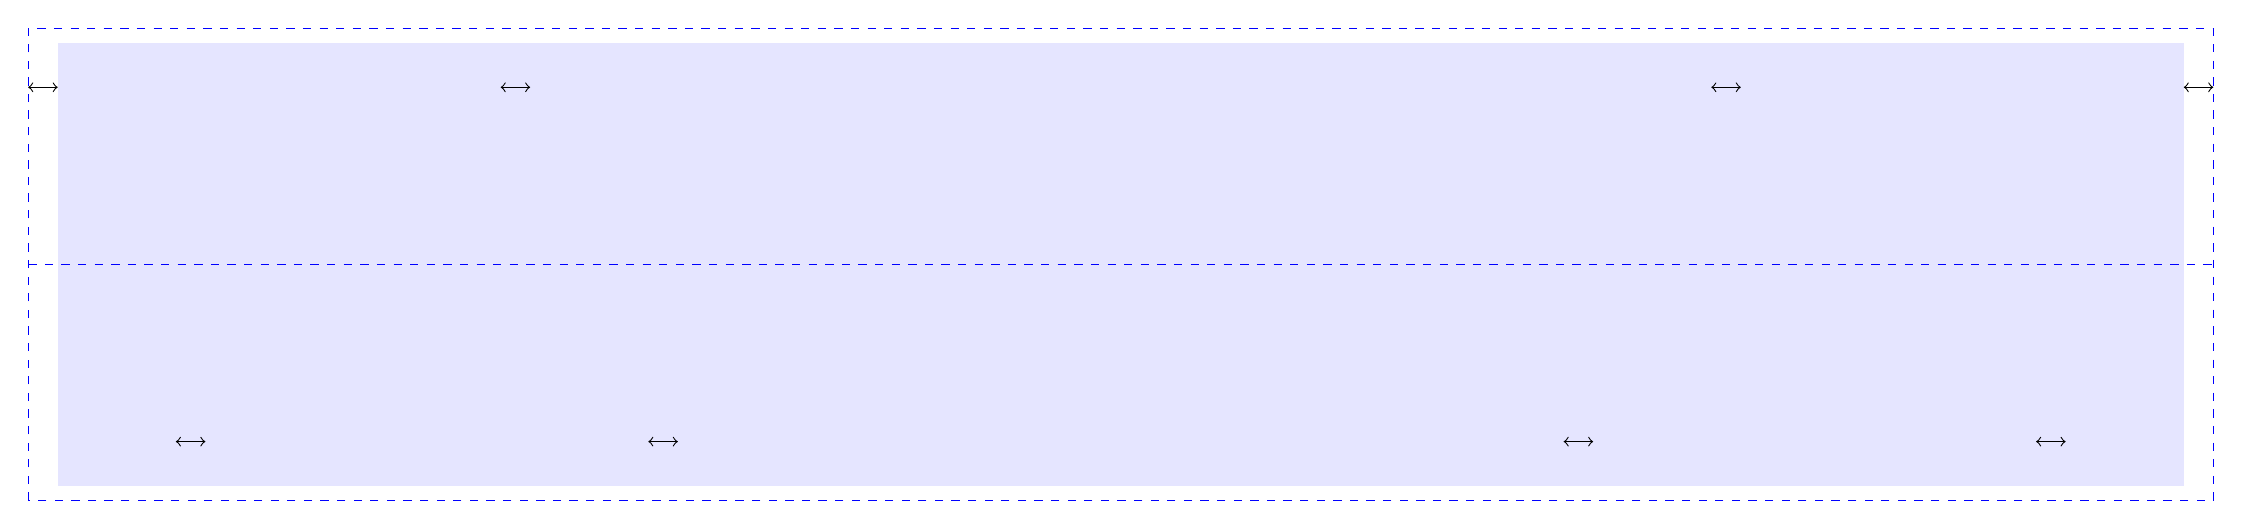
\begin{tikzpicture}[yscale=-.75,xscale=.75]

  \fill[blue!10](-15.5,3.75) rectangle (20.5,-3.75);

  \draw[dashed,blue](-16,4) rectangle(21,-4)
  (-16,0)--(21,0);

  \MathMLBox{0}{0}{1}{1}{red};

  \MathMLBox{5}{-3}{1.5}{.5}{green};
  \draw[<->] (12.5,-3) -- (13,-3);

  \MathMLBox{5}{3}{1}{.5}{green};
  \draw[<->] (10,3) -- (10.5,3);

  \begin{scope}[shift={(8,0)}]
  \MathMLBox{5}{-3}{1.5}{.5}{green};
  \draw[<->] (12.5,-3) -- (13,-3);

  \MathMLBox{5}{3}{1}{.5}{green};
  \draw[<->] (10,3) -- (10.5,3);
  \end{scope}

  \begin{scope}[shift={(-12.5,0)}]
  \MathMLBox{5}{-3}{1.5}{.5}{green};
  \draw[<->] (4.5,-3) -- (5,-3);

  \begin{scope}[shift={(2.5,0)}]
  \MathMLBox{5}{3}{1}{.5}{green};
  \draw[<->] (4.5,3) -- (5,3);
  \end{scope}
  \end{scope}

  \begin{scope}[shift={(-20.5,0)}]
  \MathMLBox{5}{-3}{1.5}{.5}{green};
  \draw[<->] (4.5,-3) -- (5,-3);

  \begin{scope}[shift={(2.5,0)}]
  \MathMLBox{5}{3}{1}{.5}{green};
  \draw[<->] (4.5,3) -- (5,3);
  \end{scope}
  \end{scope}

\end{tikzpicture}
\caption{Box model for the {\tt mmultiscripts} element}
\label{fig:MmultiscriptsBoxModel}
\end{figure}

\subsection{Tabular Math}\label{TabularMath}

The MathML specification describes tabular math as follows \cite{MathML3}:
%
\begin{quote}
Matrices, arrays and other table-like mathematical notation are marked up using
{\tt mtable}, {\tt mtr}, {\tt mlabeledtr} and {\tt mtd} elements. These
elements are similar to the table, tr and td elements of HTML, except that they
provide specialized attributes for the fine layout control necessary for
commutative diagrams, block matrices and so on.
\end{quote}
%

In the present document, we restrict ourselves to a minimal implementation
compatible with HTML tables. First the {\tt mtable} element must be treated as
a HTML table and by \cite{MathML3}, {\tt mtable} must accept a
{\tt displaystyle} attribute with default value {\tt false}. To implement that,
one may rely on the following rules for the user agent stylesheet as
suggested in section \ref{UAStylesheet}:
%
\begin{lstlisting}
  mtable {
    display: inline-table;
    mathml-math-style: inline;
  }
  mtable[displaystyle="true"] {
    mathml-math-style: display;
  }
\end{lstlisting}
%

In addition, user agents may use the following rules to emulate the {\tt frame}
attribute:
%
\begin{lstlisting}
  mtable[frame="none"] {
    border: none;
  }
  mtable[frame="solid"] {
    border: solid thin;
  }
  mtable[frame="dashed"] {
    border: dashed thin;
  }
\end{lstlisting}
%

The {\tt mtr} and {\tt mlabeledtr} elements must be treated as HTML table rows
and the label of {\tt mlabeledtr} element must be hidden by default.
The default value of {\tt rowalign} must be {\tt baseline}.
One may rely on the following rules for the user agent stylesheet
as suggested in section \ref{UAStylesheet}:

%
\begin{lstlisting}
mtr, mlabeledtr {
  display: table-row;
  vertical-align: baseline;
}
mlabeledtr > mtd:first-child {
  display: none;
}
\end{lstlisting}
%

Finally, the {\tt mtd} elements must be treated as a HTML table cell.
The default value of {\tt rowalign} must be {\tt baseline} and
the default value of {\tt colulmnalign} must be {\tt center}.
User agents may also try to approximate the default {\tt rowspacing} and
{\tt columnspacing} between cells. This can be achieved with the following CSS:

%
\begin{lstlisting}
mtd {
  display: table-cell;
  vertical-align: inherit;
  text-align: center;
  padding: 0.5ex 0.4em;
}
\end{lstlisting}
%

The {\tt mtd} element must also support the {\tt columnspan} (sic) and
{\tt rowspan} attributes. This can be implemented the same way as
the HTML {\tt colspan} and {\tt rowspan} attributes.

The layout for other tabular elements and attributes are not specified by this
document.

\subsection{Elementary Math}

Elementary Math was introduced in version 3 of the MathML specification
\cite{MathML3}:

\begin{quote}
Mathematics used in the lower grades such as two-dimensional addition,
multiplication, and long division tends to be tabular in nature. However, the
specific notations used varies among countries much more than for higher level
math. Furthermore, elementary math often presents examples in some intermediate
state and MathML must be able to capture these intermediate or intentionally
missing partial forms. Indeed, these constructs represent memory aids or
procedural guides, as much as they represent ‘mathematics’.

The elements used for basic alignments in elementary math are:

{\tt mstack}: align rows of digits and operators
{\tt msgroup}: groups rows with similar alignment
{\tt msrow}: groups digits and operators into a row
{\tt msline}: draws lines between rows of the stack
{\tt mscarries}: annotates the following row with optional borrows/carries
and/or crossouts
{\tt mscarry}: a borrow/carry and/or crossout for a single digit
{\tt mlongdiv}: specifies a divisor and a quotient for long division, along
with a stack of the intermediate computations
{\tt mfenced}
[...]
\end{quote}

This document does not define any layout algorithm for the {\tt mstack},
{\tt msgroup}, {\tt msrow}, {\tt msline}, {\tt mscarries}, {\tt mscarry} and
{\tt mlongdiv} elements.

\subsection{Enlivening Expressions}\label{maction}

The MathML specification describes {\tt maction} as follows \cite{MathML3}:
%
\begin{quote}
To provide a mechanism for binding actions to expressions, MathML provides the
maction element. This element accepts any number of sub-expressions as
arguments and the type of action that should happen is controlled by the
actiontype attribute. Only three actions are predefined by MathML, but the list
of possible actions is open.
\end{quote}
%
User agents must display at most one of the child of a {\tt maction} element.
User agents must determine the visible child as follows:
\begin{enumerate}
\item If {\tt actiontype} is {\tt toggle} and the {\tt selection} attribute
  (with default value 1) points to a valid child index
  between 1 and the number of children, then use the specified child.
\item If the {\tt actiontype} is {\tt statusline} or {\tt tooltip} then
  use the first child (if any).
\item Otherwise, the visible child is undetermined.
\end{enumerate}

For the layout algorithm described in this document, the
{\tt maction} element must be treated the same as the {\tt mrow} element
containing its visible child. If it is undetermined,
the user agent may treat the {\tt maction} element as an
empty {\tt mrow} element or as an {\tt merror} element with some relevant error
message indicating invalid or unsupported markup.

User agents may additionally provide a complete implementation of the
{\tt toggle} actiontype updating the value of the {\tt selection} attribute
after the {\tt maction} element receives a {\tt click} event.
For {\tt statusline} and {\tt tooltip} attributes, they may also display the
second child in some way when the {\tt maction} element receives a {\tt hover}
event. This document does not define how these DOM events are propagated
or how to change the default behavior.

Given the similarity with the {\tt semantics} element
described in section \ref{semantics}, it is
suggested to share the implementation of {\tt semantics} and {\tt maction}.

\subsection{Semantics and Presentation}\label{semantics}

The MathML specification describes {\tt semantics} as follows \cite{MathML3}:
%
\begin{quote}
The {\tt semantics} element is the container element that associates
annotations with a MathML expression. The semantics element has as its first
child the expression to be annotated. Any MathML expression may appear as the
first child of the semantics element. Subsequent annotation and annotation-xml
children enclose the annotations. An annotation represented in XML is enclosed
in an {\tt annotation-xml} element. An annotation represented in character data
is enclosed in an {\tt annotation} element.
[...]
\end{quote}

User agents must display at most one of the child of a {\tt semantics} element.
For example, they may always display the first child (if any) or may use this
more advanced algorithm to determine a visible child:
\begin{enumerate}
\item If the {\tt semantics} element has a first child that is any of the
  MathML elements (other than {\tt annotation} and {\tt annotation-xml})
  whose rendering is described in this document then use it as the visible
  child and stop.
\item Otherwise, check the children of the {\tt semantics} element in the DOM
  order to try and find the first child that is
  \begin{enumerate}
  \item Either an {\tt annotation} without any {\tt src} attribute.
  \item Or an {\tt annotation-xml} without any {\tt src} attribute and
    with an {\tt encoding} attribute that has value
    {\tt "application/mathml-presentation+xml"},
    {\tt "MathML-Presentation"},
    {\tt "image/svg+xml"},
    {\tt "SVG1.1"},
    {\tt "application/xhtml+xml"} or
    {\tt "text/html"}.
  \end{enumerate}
\item Otherwise, fallback to the first child (if any).
\item Otherwise, the {\tt semantics} element is empty and the visible child is
  undetermined.
\end{enumerate}

For the layout algorithm described in this document, the
{\tt annotation-xml} element must be treated the same as the {\tt mrow} element,
the {\tt annotation} element must be treated the same as the {\tt mtext}
element. The {\tt semantics} element must be treated the same as an
{\tt mrow} element containing only its visible child. If it is undetermined,
the user agent may treat the {\tt semantics} element as an
empty {\tt mrow} element or as an {\tt merror} element with some error message
indicating invalid markup.

Given the similarity with the {\tt maction} element
described in section \ref{maction}, it is
suggested to share the implementation of {\tt semantics} and {\tt maction}.
